
% LEXICAL STRESS ERRORS
%
% !TEX root = ../thesis-main.tex
%
%TODO change title? \chapter{Lexical stress errors in the IFCASL corpus}
\chapter{Lexical stress errors by French learners of German}
\label{chap:lexstress}

%\cleanchapterquote{You can’t do better design with a computer, but you can speed up your work enormously.}{Wim Crouwel}{(Graphic designer and typographer)}

%\blindtext

%\section{Stress in German vs. French }
%	\subsection{Comparative prosody}
%	\subsection{Stress ``deafness'' in French}
%	\subsection{Expected errors}
%	
	
%\TODO{Change title?}
%\section{Lexical stress errors in the IFCASL corpus} 

	
	As the previous chapter has shown, lexical stress is a challenging phenomenon for native (L1) French speakers to realize correctly in their nonnative (L2) German prosody, such that pronunciation errors with respect to lexical stress are expected to be produced frequently by this group of German learners.
%
	However, empirical studies of this type of error as produced by French learners of German are quite few in number (see \cref{sec:stress:expected,sec:targeting:frequency}), so one objective of this thesis project was to research to what extent the expected types of lexical stress errors by French speakers of German are actually produced.
	 As the IFCASL corpus (see \cref{sec:intro:ifcasl}) provides valuable data on L2 German speech produced by L1 French speakers, it is a perfect starting point for such investigations; however, given that the existing corpus annotation does not include information on lexical stress errors,
	  a subset of this corpus had to be manually annotated for such errors; the annotation and subsequent analysis of lexical errors in this data, presented in this chapter, constitute a major contribution of this thesis project.
%
	
	
	The first sections of this chapter describe the selection of material to be annotated (\cref{sec:lexstress:data}), the annotators who labeled lexical stress errors in that data (\cref{sec:lexstress:annotators}), and the method by which annotation was performed (\cref{sec:lexstress:method}). 
	
	%Once error judgments had been collected from each annotator, 
	Given the error judgments thus collected, 
	different annotators' judgments of the same utterances were compared to determine the reliability of the annotation, i.e. the agreement between annotators in terms of the labels they assigned to each utterance.
	%, which gives some indication of the general difficulty of the task of diagnosing lexical stress errors in nonnative German speech. 
	\Cref{sec:lexstress:agreement} describes this analysis of inter-annotator agreement, which aims to shed light on the following questions:
	\begin{itemize}[topsep=-1em]
	\item{How reliably can lexical stress errors be identified by
	%Can lexical stress errors be reliably identified by 
	%native German speakers 
	annotators, i.e. to what extent do the judgments of different annotators agree?  (\cref{sec:agreement:overall})}
	\item{Are there differences in how native and nonnative German speakers identify errors?  (\cref{sec:agreement:native})}
	\item{Are there differences in how 
	%expert and novice annotators (those without 
	annotators with different levels of expertise
	(annotation experience or training in phonetics/phonology) identify lexical stress errors?  (\cref{sec:agreement:expert})} 
	\end{itemize}
	%
	As \cref{sec:lexstress:agreement} will show, annotators did not always agree as to whether a given utterance exhibited a lexical stress error or not. Nevertheless, a single ``gold-standard'' label for each utterance had to be selected; \cref{sec:agreement:gold} describes how this was accomplished in cases of disagreement.
	
	Finally, given the gold-standard labels for each utterance, the distribution of lexical stress errors in the annotated data was analyzed; the following questions guided this analysis, which is detailed in \cref{sec:lexstress:results}.
	\begin{itemize}[topsep=-1em]
	\item{Are lexical stress errors observed frequently in the IFCASL data? (\cref{sec:results:overall})}
		\item{Are lexical stress errors observed more frequently with certain word types than with others?  (\cref{sec:results:wordtype})}
	\item{Is there a difference in the frequency of these errors among different groups of speakers, i.e. in terms of skill level, age, or gender? (\cref{sec:results:level,sec:results:agegender})}
	%or in different contexts (e.g. after hearing a native speaker produce the word)?  (\cref{sec:results:level,sec:results:agegender,sec:results:condition})}
	%\item{How frequently do technical problems interfere with determining whether an error was made?  (\cref{sec:results:techproblems})}
	\end{itemize}
	%	
	In addition to enabling this error distribution analysis, the annotated data compiled as described in this chapter also enables the use of supervised machine learning methods for the automatic detection of lexical stress errors, which is the subject of \cref{sec:diag:classification}).
	
	%\subsection{Data}
	\section{Data}
	\label{sec:lexstress:data}
	
	The IFCASL corpus \citep{Trouvain2013,Fauth2014}, introduced in \cref{sec:intro:ifcasl}, contains recordings of native and nonnative speech in French and German, and is thus a invaluable resource for research on pronunciation errors in this language pair, with the subset of the corpus containing L2 German speech by L1 French speakers (henceforth IFCASL-FG) being most relevant to the work reported in this thesis. As described in \cref{sec:intro:ifcasl}, speakers of varying ages, genders, and German proficiency levels are represented in the IFCASL-FG corpus; the exact number and characteristics of these speakers are presented in \cref{tab:data:speakers}.
	
	
		\begin{table}
			\centering
			\caption[Speakers in the annotated dataset]{Number of speakers in the portion of the IFCASL-FG corpus annotated for lexical stress, in terms of speakers' age, gender, and proficiency level}
			\begin{tabular}{lrrrrr}
			\toprule
			\multirow{2}{*}{Age/gender}	&	\multicolumn{4}{c}{Proficiency level} &\multirow{2}{*}{\textbf{Totals}}\\
			\cmidrule(lr){2-5}
		& A2	&	B1	&	B2	&	C1	&		\\
			\midrule
Boy	&	11	&	0	&	0	&	0	&	\textbf{11}	\\
Girl	&	1	&	1	&	0	&	0	&	\textbf{2}	\\
Man	&	7	&	4	&	3	&	7	&	\textbf{21}	\\
Woman	&	5	&	5	&	3	&	9	&	\textbf{22}	\\
			%\midrule
\textbf{Totals}	&	\textbf{24}	&	\textbf{10}	&	\textbf{6}	&	\textbf{16}	&	\textbf{56}	\\
			\bottomrule
			\end{tabular}
			\label{tab:data:speakers}
		\end{table}
	
	
	The subset of IFCASL-FG selected for the lexical stress error annotation undertaken in this work, henceforth referred to simply as ``the dataset,''
	 consists of utterances of twelve word types (see \cref{tab:bisyllwords}), each of which is bisyllabic and canonically has its primary stress on the initial syllable. These characteristics were chosen deliberately: the selected words are bisyllabic because this simplifies comparison between stressed and unstressed syllables, and they are initial-stress because this is the stress pattern which native (L1) French speakers are expected to have the most difficulty producing in German, given the fixed final-position stress and final lengthening in French (see \cref{sec:stress:expected}). 
	
	Though previous work on lexical stress errors in L2 speech has often dealt with words uttered in isolation (e.g. \cite{Bonneau2011}), this work deals with word utterances extracted from longer utterances of complete sentences; as \textcite[p.~6]{Neri2002} point out, for relevance to real communication it is important that CAPT systems address connected speech. The word's position in the carrier phrase/sentence was not taken into account; although it could be hypothesized that phrase position would have an effect on lexical stress realization by native French speakers, given the phenomenon of phrasal accent in French (see \cref{sec:stress:french}), \textcite{Michaux2013} found no effect of phrase position on French speakers' realization of words in Dutch. Given the similarities in the lexical stress systems of Dutch and German with respect to French, no such phrase-level effect is therefore expected here, though investigation of the effect of phrase or sentence position on stress realization could be an interesting direction for future work.
	
	In the IFCASL corpus recordings, sentences containing these words were read aloud by both L1 and L2 (L1 French) German speakers, as mentioned in \cref{sec:intro:ifcasl}. Here, only the L2 utterances were manually annotated; it is assumed that the L1 German speakers always realize lexical stress correctly, so the utterances of the selected word types in the native German subset of the IFCASL corpus (IFCASL-GG) were not manually annotated, but rather automatically labeled as correct realizations (see \cref{sec:classification:datamethod}).
	
%	\TODO{\textit{take out?}} As mentioned in \cref{sec:intro:ifcasl}, the IFCASL recordings were performed under two conditions: the ``Sentence Read'' (SR) condition, in which the L2 speaker is simply  presented with the text of the sentence and asked to record themselves reading it aloud, and the ``Sentence Heard'' (SH) condition, in which the L2 speaker is asked to listen to an utterance of the sentence by an L1 German speaker before recording their own utterance. The sub-corpus for annotation includes recordings from both conditions, though the majority are from the SR condition. \TODO{reason for imbalance}
	
	To compile the dataset, utterances (tokens) of each word as produced by over 50 L2 speakers were extracted from the recordings automatically with Praat \parencite{Boersma2014}, using extraction times (start and end points of word utterances) taken from the word-level segmentation of each sentence utterance automatically obtained by forced alignment (see \cref{sec:diag:segmentation}).
	\Cref{tab:bisyllwords} lists the exact number of tokens available for each word type. In total, 
	%669 
	668 word tokens were annotated for lexical stress errors. 
	%Four 
	Five tokens had to be excluded from the data, as disfluencies in the sentence utterance (e.g. false starts or repetitions of the target word) prevented the automatic extraction of the word utterance from the sentence as a whole. In a fully-fledged student-facing CAPT system, such disfluencies would need to be dealt with accordingly, e.g. by means of a pre-processing step which analyzes the student's utterance for possible disfluencies and compensates for any that are detected by, for example, prompting the student to re-record their utterance. However, detecting disfluencies in speech, especially nonnative speech, is a challenging problem under active research 
	(see \cref{sec:capt:auto}),
	%(see e.g. \cite{Bonneau2012,Orosanu2012}), 
	and the development of a  disfluency-aware system is outside the scope of this thesis project; therefore, this work presupposes that no disfluencies exist in the student's utterance, and the handful of disfluent tokens have been excluded from the error-annotated sub-corpus described here.
	
	\begin{table}[htb]
		\centering
		\caption[Word types annotated for lexical stress errors]{The twelve bisyllabic initial-stress words types selected from the IFCASL corpus for lexical stress error annotation. 
		%The orthographic form (text) of each word type is presented in the leftmost column, followed by its canonical pronunciation (e.g. as found in a pronunciation dictionary). 
		Canonical pronunciations for each word type are given in SAMPA notation (\url{http://www.phon.ucl.ac.uk/home/sampa}), with phonemes separated by a space and syllables separated by a period (\texttt{.}); canonical lexical stress is not marked, as all of the listed word types have primary stress on the initial syllable. 
		%Parts of speech are abbreviated as n. (noun), v. (verb) and pro. (pronoun). 
		The rightmost column lists the number of tokens (utterances) of each word type included in the annotated dataset.
		}
%		\begin{tabular}{llll}
%		Flagge & Ringen & Tschechen & halten \\
%		M\"{o}rder & Tatort & Fr\"{u}hling & fliegen \\
%		Pollen & manche & E-mail & tragen \\
%		\end{tabular}
		
		%\begin{tabularx}{\textwidth}{llXlX}
		\begin{tabular}{llllc}
		\toprule
		
		Orthography & 
		%Canonical \linebreak 
		Pronunciation & 
		Part of speech & 
		English meaning & 
		%Recording condition \TODO{remove?}& 
		Tokens\\%\linebreak annotated\\
		
		\midrule
		E-mail		&	\texttt{i:~.~m eI l} 		&	noun &	e-mail %&	SR 	
			&	56	\\
		Flagge		&	\texttt{f l a~.~g @} 		&	noun &	 flag %&	SH	
			&	55	\\
		fliegen		&	\texttt{f l i:~.~g =n} 	&	verb &	to fly %&	SR		
			& 56	\\
		Frühling	&	\texttt{f r y:~.~l I N} 		& noun	&	spring \newline (season) %&	SR		
			&	56	\\
		halten		&	\texttt{h a l~.~t =n}		&	verb &	to hold %&	SR 	
			&	56	\\
		manche	&	\texttt{m a n~.~C @} 		&	pronoun &	some %& 	SR 	
			&	56	\\
		Mörder		&	\texttt{m 96~.~d 6}		&	noun &	murderer %&	SR 	
			&	56	\\
		Pollen		&	\texttt{p O~.~l @ n} 		&	noun &	pollen %&	SR 	
			& 	55	\\
		Ringen		&	\texttt{r I N~.~@ n}		&	noun &	rings %&	SH	
			&	55	\\
		Tatort		&	\texttt{t a:~t~.~?~O6 t}	&	noun &	crime scene %& 	SR 	
			&	56	\\
		tragen		&	\texttt{t r a:~.~g =n} 	&	verb &	to wear %&	SH	
			&	55	\\
		Tschechen	& \texttt{tS E~.~C =n}	& noun	&	Czechs	%&	SR		
			& 56	\\
		\bottomrule
		\end{tabular}
		\label{tab:bisyllwords}
	\end{table}
	
	\section{Annotators}
	\label{sec:lexstress:annotators}
	
	A total of 15 annotators participated in the annotation of this dataset,
	%\TODO{\textit{remove?:} over the course of 2 months}, 
	each of whom is listed in \cref{tab:annotators} (by an arbitrary identifier, to preserve anonymity).
	As \cref{tab:annotators} shows, the annotators varied with respect to their native language, as well as with respect to their level of expertise in phonetics/phonology/linguistic annotation. 
	 
	 % Nativeness
	Of the 15 annotators, the majority (12) are native German speakers, and three are nonnative (L2) speakers: two are native speakers of American English, and one is a native Hebrew speaker. The L2 German speakers all have some knowledge of German as L2, though the exact German proficiency levels of these annotators are unknown.
	
	% Expertise
	In terms of expertise, the annotators can broadly be categorized into three groups: 
	\begin{itemize}[itemsep=0pt, topsep=-1em, partopsep=0pt]
	\item{\textit{expert} annotators are professional researchers with a thorough understanding of phonetics/phonology and extensive experience in annotating speech data}
	\item{\textit{intermediate} annotators are university students enrolled in an experimental phonology course,
	% \textit{is that true of Frankfurt students too?}}, 
	and have some training in phonetics/phonology and/or experience annotating speech data}
	\item{\textit{novice} annotators have negligible training in phonetics/phonology and little, if any, experience annotating speech data}
	\end{itemize}
	As shown in \cref{tab:annotators}, the majority of annotators (10 out of 15) fall into the \textit{intermediate} group; two annotators can be considered \textit{expert}, and there are three \textit{novice} annotators.
	
	
	\begin{table}[p]
		\centering
		\caption[Annotators]{Annotators participating in the lexical stress error annotation. The anonymous identifier (ID), native language (L1) and expertise level of each annotator are presented, along with the word types each was asked to annotate and the number of usable token annotations by that participant for each word.}
		
		\begin{tabularx}{\textwidth}{lllX}
		\toprule
		ID & L1 & Expertise & Word types annotated (nb. of usable tokens) \\
		\midrule
		%Frank	FZ 
		A	&	German	& expert & Flagge (55),  Ringen (55), Tschechen (56) \\
		

		%Jeanin JJ	
		H & German & expert &		 fliegen (56), Fr\"{u}hling (56),  Pollen (55) \\		
		
		
		%Raphael	RM	
		B	&	German	& intermediate & 	halten (56),  M\"{o}rder (56),     Tatort (56) \\
		
		

		%Diana	DA 
		D &	German & intermediate &		Flagge (49),  Pollen (53), Ringen (49)	 %\TODO{FALSE}   
		\\
		

		
		%Sarah	SC
		F & 	German	 & intermediate & 	 fliegen (56), Fr\"{u}hling (56), Tatort (56)	 \\
		

		

		%Dilber	DB 
		I & 	German & intermediate &		halten (56), Ringen (55), Tschechen (56)	 \\
		
		%Christine	CM
		J &	German	 & intermediate & Fr\"{u}hling (56), M\"{o}rder (56),    Tatort (56) \\
		

		
		
		%Maya	ML
		M & 	German	 & intermediate & Fr\"{u}hling (56), Ringen (54),   tragen (55)	 \\
		
		%Steffen	SB
		%Q
		O	& German	 & intermediate & manche (56), Mörder (56),    tragen (55) \\




		
		%Tobias	TB	
		%P
		C & German & novice & 	 E-mail (56), halten (56),  Pollen (55)	 \\
		
		
		%Marc	MS	
		L & German	 & novice & E-mail (56), Flagge (54),  Tatort (56) \\
		

		
		%Lisa	LB	
		N & German	& novice & fliegen (56),  manche (56), Tschechen (56)	 \\
		
		
		
		%Yoav	YB	 
		G & Hebrew	& intermediate & Flagge (20), 	fliegen (0),  Pollen (0)	 %\TODO{FALSE}   
		\\		

		%Patrick	PC 
		E & English (US)	& intermediate & 	halten (56),  M\"{o}rder (56), Tschechen (56) 	 \\

		%Anjana	AV	
		K & English (US)	& intermediate &  E-mail (56), Flagge (55),	    fliegen (56),  manche (56),   Pollen (55),   tragen (55) \\		
		



		\bottomrule
		\end{tabularx}
		\label{tab:annotators}
	\end{table}
	
	
	
	
	Each annotator was assigned three word types to annotate in a single session, with the exception of one annotator who was assigned six word types over two sessions (see \cref{sec:lexstress:method} for a description of an annotation session). \Cref{tab:annotators} lists the word types assigned to each annotator, along with the number of tokens labeled for each type. Some judgments by annotators D and G had to be excluded from the analysis due to technical problems; the token counts for each annotator in \cref{tab:annotators} reflect only their usable judgments. 
	
	Word types were assigned to ensure that each was annotated by at least two native German speakers, and to maximize the amount of overlap between annotators in order to obtain as many pairwise measures of annotator agreement as possible (see \cref{sec:lexstress:agreement} for a discussion of inter-annotator agreement); \cref{tab:annotatorsbyword} lists the number of annotators for each word type.
	
	\begin{table}[p]
		\centering
		\caption[Number of annotators assigned to each word type]{Number of annotators assigned to each word type, in terms of the native language and expertise groups described in this section. The rightmost column gives the total number of annotators assigned to each word type.}
		\begin{tabular}{lcccccc}
		\toprule
		%Word type
		&		Native %annotators 
		& 	Nonnative %annotators 
		& Expert
		& Intermediate
		& Novice
		& Total %annotators 
		\\
		\midrule
		E-mail			& 2 	& 1 	&	0	&	1	&	2	& 3 \\
		Flagge			& 3	& 2	&	1	&	3	&	1	& 5 \\
		fliegen			& 3	& 1	&	1	&	2	&	1	& 4 \\
		Frühling		& 4	& 0	&	1	&	3	&	0	& 4 \\
		halten			& 3	& 1	&	0	&	3	&	1	& 4 \\
		manche		& 2	& 1	&	0	&	2	&	1	& 3 \\
		Mörder 		& 3	& 1	&	0	&	4	&	0	& 4 \\
		Pollen			& 3	& 1	&	1	&	2	&	1	& 4 \\
		Ringen			& 4	& 0	&	1	&	3	&	0	& 4 \\
		Tatort			& 4	& 0	&	0	&	3	&	1	& 4 \\
		tragen			& 2	& 1	&	0	&	3	&	0	& 3 \\
		Tschechen 	& 3	& 1	&	1	&	2	&	1	& 4 \\
		\bottomrule
		\end{tabular}
		\label{tab:annotatorsbyword}
	\end{table}
	
	
	
	%\subsection{Annotation method}
	\section{Annotation method}
	\label{sec:lexstress:method}

	The annotation task consisted of assigning one of the following labels to 
	%the lexical stress realization in 
	each token of the selected word types, i.e. each utterance of each word by each L1 French speaker in the corpus:
	
	\begin{itemize}
	\item{[correct]: the speaker audibly stressed the lexically stressed (initial) syllable}
	\item{[incorrect]: the speaker audibly stressed the lexically unstressed (final) syllable}
	\item{[none]: the speaker did not clearly stress either syllable, i.e. did not audibly differentiate stressed and unstressed syllables, or the annotator was unable to determine which syllable was stressed}
	\item{[bad\_nsylls]: the speaker pronounced the word with an incorrect number of syllables (i.e. by inserting or deleting a syllable), rendering it impossible to judge whether stress was realized correctly or not}
	\item{[bad\_audio]: a problem with the audio file (e.g. noise in the signal or very inaccurate segmentation) interfered with the annotator's ability to judge the stress realization}
	 \end{itemize}
	
	Annotation proceeded by means of a graphical tool scripted in Praat \parencite{Boersma2014}, the main interface of which is shown in \cref{fig:annotationtool}. At the top, a word's text is displayed, along with the IFCASL corpus ID number of the speaker whose utterance of that word will be annotated (this number is only relevant for the annotator insofar as changes in its value inform the annotator that the speaker is changing from utterance to utterance). The recording of the word
%, extracted automatically from the utterance of the entire sentence using the boundaries of the forced-alignment segmentation, 
is played once automatically; the annotator may then choose to click one of the green buttons to play the word again, or play the recording of the entire sentence, as many times as they wish. Once the annotator has judged the accuracy of the lexical stress realization in this utterance, they log that judgment by clicking one of the gray buttons. The annotator is then automatically advanced to the next utterance, with the counts in the lower right corner tracking their progress towards the total number of tokens to be annotated. 

A single annotation session consisted of annotating all tokens of three word types, and lasted approximately 15 minutes. As mentioned in \cref{sec:lexstress:annotators} above, each annotator participated in one session, with the exception of annotator K who participated in two sessions (separated by several days) and annotated a total of six word types.
	
		\begin{figure}[t]
			\centering
			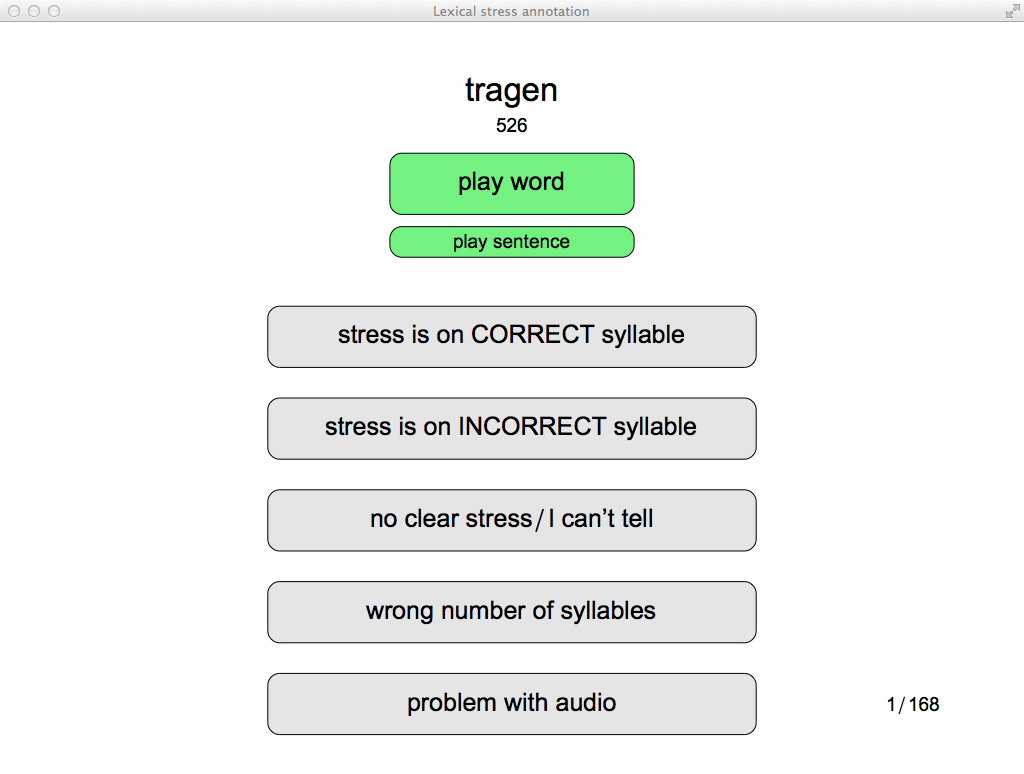
\includegraphics[width=\textwidth]{img/screenshots/AnnotationTool}
			\caption[A screenshot of the graphical annotation tool scripted in Praat.]{A screenshot of the graphical annotation tool scripted in Praat. Green buttons allow the annotator to listen to  the word and sentence utterances. Gray buttons allow the annotator to record their judgment of stress accuracy; from top to bottom, the buttons correspond to the labels [correct], [incorrect], [none], [bad\_nsylls], and [bad\_audio].}
			\label{fig:annotationtool}
		\end{figure}
		
		
		%\vspace{2em}
		
		The lexical stress error 
		annotations collected in this manner for each token (utterance) in the dataset enable two important contributions of this thesis, described in the following sections. 
		First, the multiple annotations for each token from different annotators permit an analysis of inter-annotator agreement with regard to the identification of lexical stress errors; \cref{sec:lexstress:agreement} presents this analysis, along with statistics on the relative frequencies with which the five labels were selected by annotators from the different L1 and expertise groups described in \cref{sec:lexstress:annotators}.
		Secondly, and perhaps more importantly, the errors identified by these annotators in the data extracted from the IFCASL corpus enable an analysis of the frequency of lexical stress errors in the speech of L1 French learners of German as L2; this is the subject of \cref{sec:lexstress:results}.
		
	
	\section{Inter-annotator agreement}
	\label{sec:lexstress:agreement}	
	
	To create a useful CAPT system for lexical stress errors in nonnative German, i.e. to automatically detect whether a student has made a lexical stress error in a given utterance, it is helpful to have an understanding of the difficulty of the error-detection task, not only for machines but for humans. It is therefore useful to analyze the collected stress accuracy judgments in terms of inter-annotator agreement, in order to gain insight into the nature of the challenge this task presents. If it is uncommon for human annotators to agree about whether a given lexical stress realization is correct or incorrect, this may indicate that  identifying lexical stress errors is a challenging task, and one which an automatic system should also be expected to have difficulty with. If, on the other hand, human annotators are generally in strong agreement, this may reflect a lower level of difficulty, and give reason to judge the performance of an automatic system by a higher standard.  
	
	As stated in the previous section,
	%\cref{sec:lexstress:data}, 
	lexical stress realizations in a total of 
	%669 
	668 word utterances were each assigned to one of five classes by multiple annotators, based on whether the annotator judged the production to have correctly placed stress, incorrectly placed stress, no clear stress placement, or other problems which prevented the annotator from making a judgment about the lexical stress accuracy. 
	For 268 of these utterances, i.e. approximately 40\% of the dataset, there was perfect agreement among annotators as to which of the five possible labels was most appropriate. This means that for the majority of the dataset (400 utterances, or approximately 60\%), at least one annotator's judgment diverged from that of the other(s) who labeled the same utterance.
	
	
	To make sense of these differences,  
	%and obtain a clearer picture of inter-annotator agreement in the error-detection task, the agreement between these judgments 
	agreement in label assignments was calculated for each pair of annotators who overlapped, i.e. labeled any of the same tokens. 
	\TODO{matrix of pairwise tokens in common (or just x/o to show which annotators overlapped?}
	%This section describes how this agreement was calculated, and the following sections \cref{sec:agreement:overall, sec:agreement:native, sec:agreement:expertise} present an analysis of the resulting inter-annotator agreement statistics. Finally, 
		Two metrics were used to quantify agreement between a pair of annotators: the simple percentage of observed agreement, and Cohen's Kappa ($\kappa$) statistic; the following paragraphs describe how these are computed. In the analysis presented in \cref{sec:agreement:overall,sec:agreement:native,sec:agreement:expert}, both metrics are presented together in the hopes of providing a more comprehensive picture of inter-annotator agreement than either can convey alone.  
		
		
		For a given pair of annotators, percentage agreement is calculated as the number of tokens to which both annotators assigned the same label, divided by the total number of tokens labeled by both annotators. Possible values for percentage agreement range from 0\%, representing complete disagreement between annotators, to 100\%, representing complete agreement. This simple metric ignores the probability of annotators agreeing by chance, and therefore may give a somewhat optimistic picture of inter-annotator agreement, but nevertheless serves as a basic, easy-to-interpret preliminary indication of the reliability of the collected judgments.
		
		To account for chance agreements not captured by the simple percentage of agreement, a second, more robust measure of inter-annotator agreement, Cohen's $\kappa$ statistic \citep{Cohen1960}, was also calculated for each pair of annotators. For a given pair of annotators who have labeled the same tokens, $\kappa$ is computed as
		\[
		\kappa = \frac{p_a-p_c}{1-p_c}
		\]
		where $p_a$ is the proportion of tokens assigned the same label by both annotators (i.e. the simple percentage agreement just described) and $p_c$ is the proportion of tokens which can be expected to receive the same label from both annotators purely by chance. The latter thus represents the probability of the two annotators agreeing by chance, and is calculated for a pair of annotators $A$ and $B$ as
		\[
		p_c = \sum_{s \in S} p_A(s) \times p_B(s)
		\]
		where $s$ is one of the stress judgments in the set of possible labels $S$:
		\[S = \{\text{[correct]}, \text{[incorrect]}, \text{[none]}, \text{[bad\_nsylls]}, \text{[bad\_audio]}\}\]
		and $p_A(s)$ is the proportion of tokens assigned the label $s$ by annotator $A$, calculated as the number of tokens assigned label $s$ by annotator $A$ divided by the total number of tokens labeled by annotator $A$; $p_B(s)$ is calculated in the same way for annotator $B$.
		%and $p_A(s)$ and $p_B(s)$ are the proportion of tokens assigned the label $s$ by annotators $A$ and $B$, respectively. The value of $p_A(s)$ is calculated as the number of tokens assigned label $s$ by annotator $A$ divided by the total number of tokens labeled by annotator $A$. 
		As $\kappa$ thus accounts for the probability of two annotators assigning a token the same label purely by chance, it provides a more conservative measure of inter-annotator agreement. A $\kappa$ value of 0 indicates that the annotators do not agree any more than would be expected by chance. If agreement between annotators is less than chance, $\kappa$ will take a value below 0. The maximum possible value of $\kappa$ is 1.00, which indicates perfect agreement between annotators.
		

		%\TODO{Anything else to say here?}
		
		\subsection{Overall agreement}
		\label{sec:agreement:overall}
		
		To obtain an overall measure of inter-annotator agreement for this lexical stress assessment task, the agreement between each pair of overlapping annotators was quantified by the metrics discussed in the previous section, and the minimum, median, mean, and maximum values over all pairwise comparisons were computed; these values are given in \cref{tab:agreement:overall}.
	Though this provides a rather coarse-grained picture of the overall agreement, this simple analysis already points to a few interesting observations. First of all, the mean and median percentage agreement are near 55\%, indicating that, roughly speaking, annotators agree just slightly more often than they disagree.
	%The $\kappa$ values are somewhat more difficult to interpret, but i
	Turning to the $\kappa$ values, given that $\kappa = 0$ represents agreement purely by chance while $k = 1$ represents perfect, meaningful agreement, the fact that the mean and median $\kappa$ values between annotators are somewhere near 0.25 indicates that the agreement observed between annotators is closer to what would be expected simply by chance than to agreement that would indicate highly reliable annotations, and signifies ``fair'' agreement between annotators according to the thresholds proposed by \textcite{Landis1977}. Examination of the minimum and maximum values reveals that while some pairs of annotators seem to exhibit ``substantial'' agreement, 
	%removing this because it's not certain that these numbers correspond to the same pair:
	%with one pair reaching over 80\% agreement and a $\kappa$ over 0.6, 
	indicating reasonably reliable judgments, other pairs have ``poor'' agreement; in one case, with 23.21\% agreement, the annotators seem to be closer to perfect disagreement than perfect agreement, and the corresponding $\kappa$ being below zero indicates that they agreed even (slightly) less than one would expect if they were merely labeling utterances randomly. 
	
	
	

		\begin{table}[tb]
			\centering
			\caption{Overall pairwise agreement between annotators}
			\begin{tabular}{lrr}
			\toprule
				&	\% Agreement	&	Cohen's $\kappa$	\\
			\midrule
Mean		&	54.92\%	&	0.23	\\
Maximum	&	83.93\%	&	0.61	\\
Median		&	55.36\%	&	0.26	\\
Minimum	&	23.21\%	&	-0.01	\\
			\bottomrule
			\end{tabular}						
			
%			\begin{tabular}{lrrrr}
%				\toprule
%				Agreement measure &	Minimum	& Median &	 Maximum &	 Mean\\
%				\midrule
%				Percentage agreement &	23.21\%	& 55.36\%	& 83.93\%	& 54.92\% \\
%				Cohen's $\kappa$ & 	-0.01	& 0.26	& 0.61	& 0.23 \\
%				\bottomrule
%			\end{tabular}
			\label{tab:agreement:overall}
		\end{table}
	
	
	
	It seems, then, that there may be stark differences in reliability from annotator to annotator. Analysis of the set of pairwise comparisons between a given annotator and all overlapping annotators provides more insight into that annotator's individual reliability. \Cref{fig:agreement:annotators} illustrates the pairwise agreements involving each of the 15 annotators. \TODO{table of percent/kappa min/avg/max by annotator, since graphs are difficult to read precisely?} Evidently, there is noticeable variation from annotator to annotator, with some annotators (e.g. C, with a mean percentage agreement of \TODO{X} and a mean $\kappa$ of \TODO{Y}) appearing generally more reliable than others (e.g. F, with mean \%=\TODO{X} and mean $\kappa$=\TODO{Y}).  \TODO{stat. significance?} However, these figures should be interpreted with caution because they do not account for differences in the number of overlapping annotators/tokens available for each annotator \TODO{reference overlap table}. 
	%nonetheless, it seems that there is indeed some noticeable variation from annotator to annotator. \TODO{finish this paragraph}
		
		
		\begin{figure}[p]
			\centering
			
%			\begin{subfigure}[b]{\textwidth}
%				\centering
%				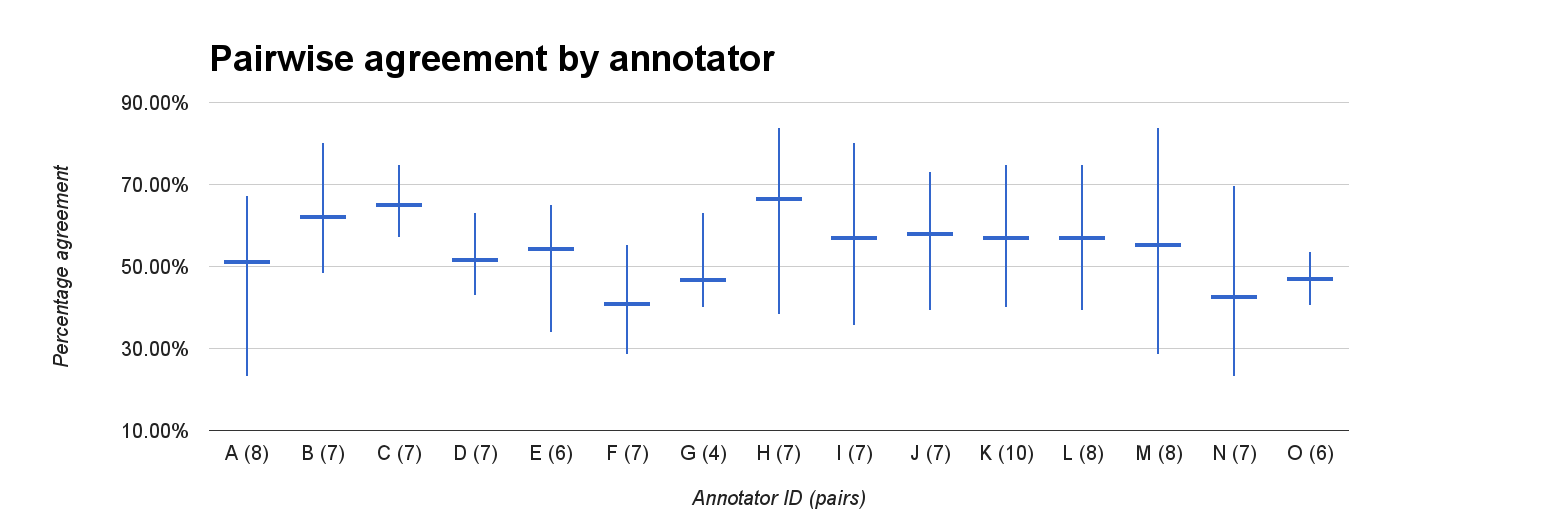
\includegraphics[width=\textwidth]{img/annotation/pairAgreeAnnotators}
%				\caption{Percent agreement}
%				\label{fig:agreement:annotators:pct}
%			\end{subfigure}%
			
%			\begin{subfigure}[b]{\textwidth}
%				\centering
%				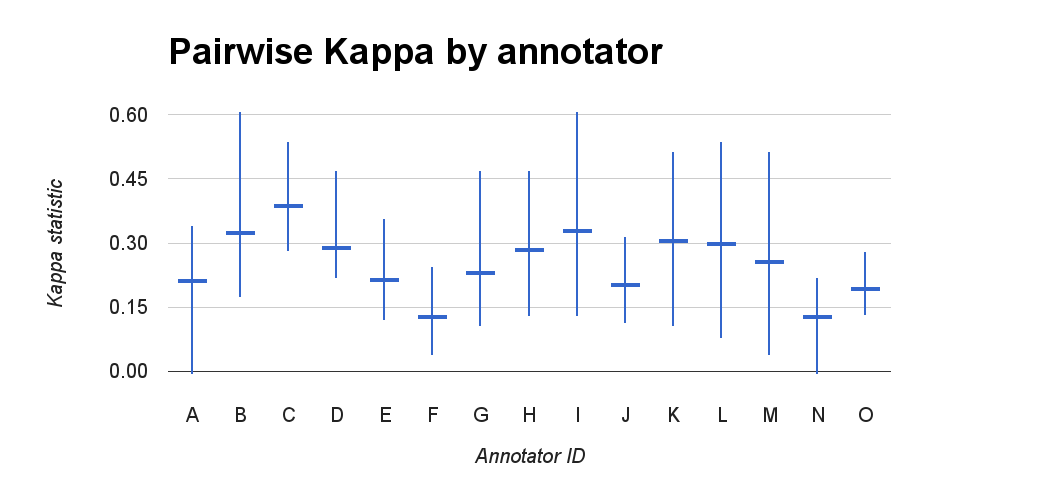
\includegraphics[width=\textwidth]{img/annotation/pairKappaAnnotators}
%				\caption{Cohen's Kappa statistic}
%				\label{fig:agreement:annotators:k}
%			\end{subfigure}%

			

			
			\begin{subfigure}{\textwidth}
				\centering
				\caption{Pairwise percentage agreement by annotator}
				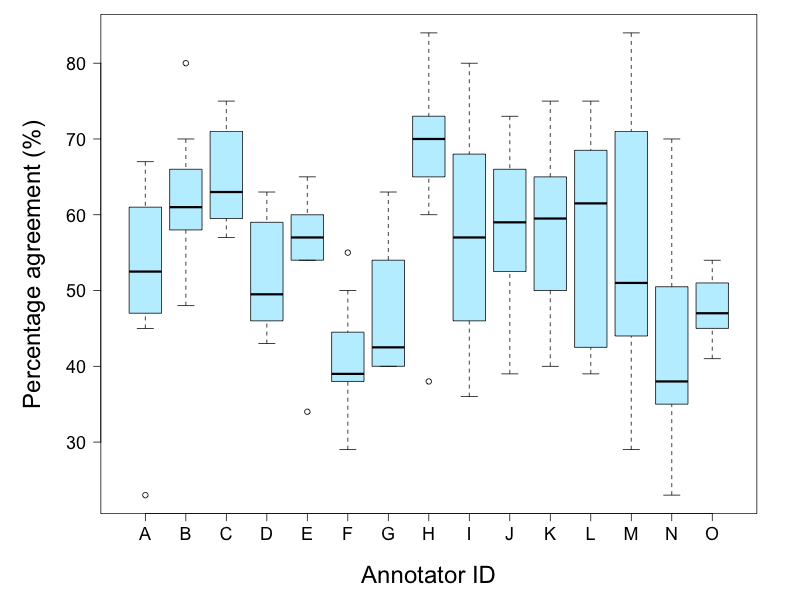
\includegraphics[width=.9\textwidth]{img/plots/pairwisePercentageByAnnotator-noTitle}
				\label{fig:agreement:annotators:pct}
			\end{subfigure}%

			\vspace{2em}			
			
			\begin{subfigure}{\textwidth}
				\centering
				\caption{Pairwise $\kappa$ by annotator}
				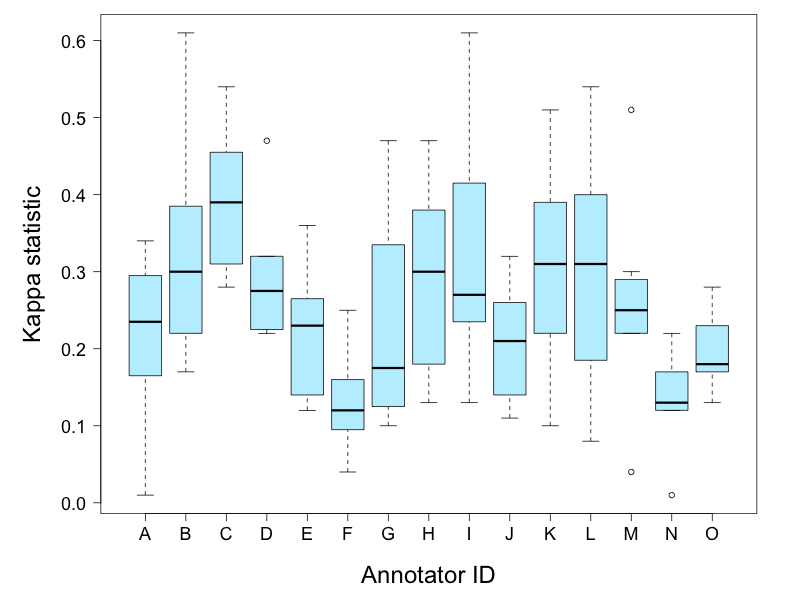
\includegraphics[width=.9\textwidth]{img/plots/pairwiseKappaByAnnotator-noTitle}
				\label{fig:agreement:annotators:k}
			\end{subfigure}%
			
			\vspace{1em}	

			\caption[Pairwise agreement statistics by annotator]{Each annotator's pairwise agreement with all other annotators with whom they overlapped.
			Horizontal lines represent median values. Colored boxes extend from the first quartile to the third quartile, and thus represent the Inter Quartile Range (IQR). Whiskers extend to the minimum and maximum values within 1.58 IQR of the first and third quartiles, respectively, and roughly represent a 95\% confidence interval around the median. 
			 Outliers that fall outside of the IQR by a distance of more than approximately 1.5$\times$IQR  are represented by circles.%
			%Numbers in parentheses indicate the number of pairwise comparisons involving each annotator. The bottom of each vertical bar represents the minimum pairwise value, the top the maximum. Horizontal bars indicate mean pairwise values.
			}
			
			\label{fig:agreement:annotators}
		\end{figure}
		
		It is also of interest to analyze the overall inter-annotator agreement for each word type in the dataset (see \cref{tab:bisyllwords} for the list of annotated word types). \TODO{table of  min/med/max/mean by word?} As \cref{fig:agreement:words} illustrates, there are noticeable differences between word types, with annotators exhibiting relatively high agreement on certain words (e.g. \textit{E-mail}, \textit{halten}, and \textit{Pollen}), while for other words (e.g. \textit{manche} and \textit{Ringen}) agreement values are closer to chance. \TODO{DISCUSSION (reference error breakdown by word in sec:results:overall}
		
		
		\begin{figure}[phtb]
			\centering
			
%			\begin{subfigure}[b]{\textwidth}
%				\centering
%				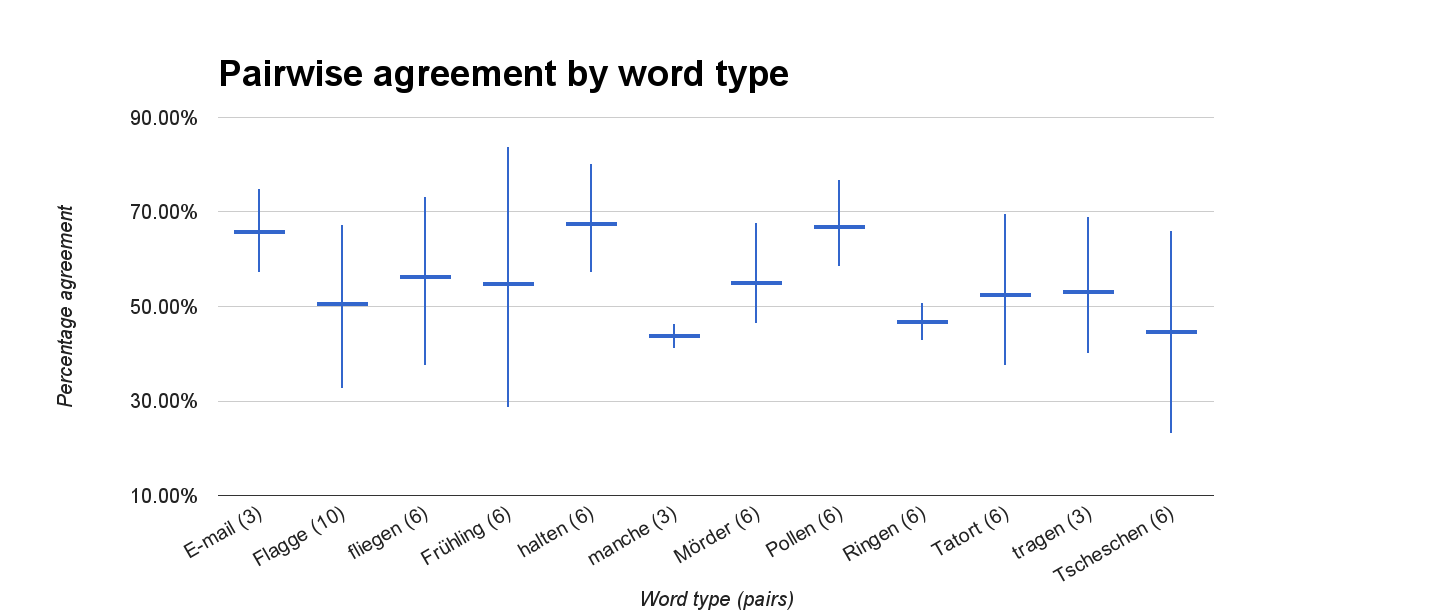
\includegraphics[width=\textwidth]{img/annotation/pairAgreeWords}
%				\caption{Percent agreement}
%				\label{fig:agreement:words:pct}
%			\end{subfigure}%
%			
%			\begin{subfigure}[b]{\textwidth}
%				\centering
%				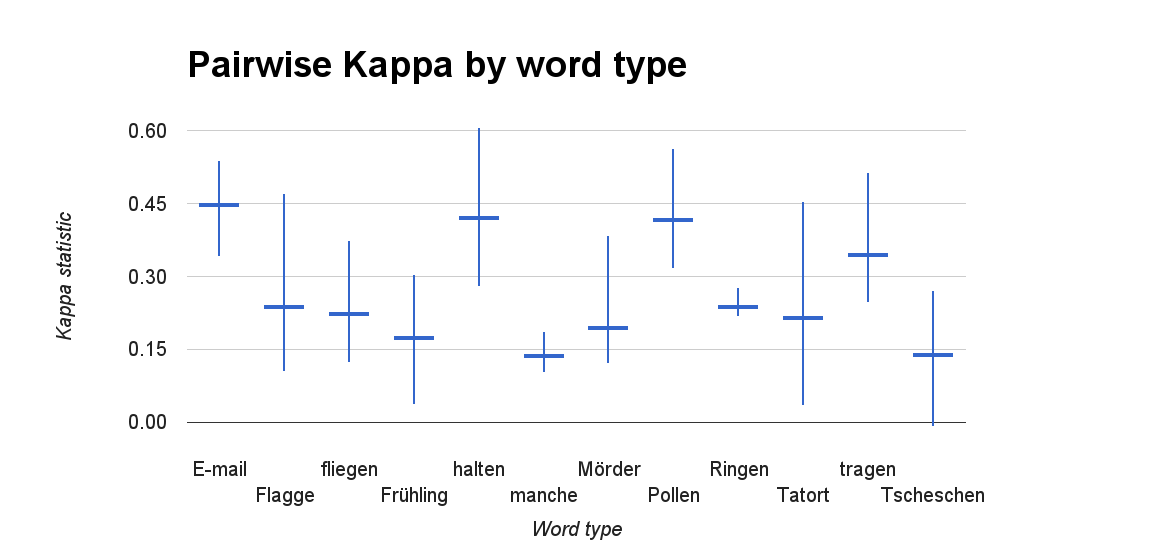
\includegraphics[width=\textwidth]{img/annotation/pairKappaWords}
%				\caption{Cohen's Kappa statistic}
%				\label{fig:agreement:words:k}
%			\end{subfigure}%

					
			
			\begin{subfigure}{\textwidth}
				\centering
				\caption{Pairwise percentage agreement by word type}
				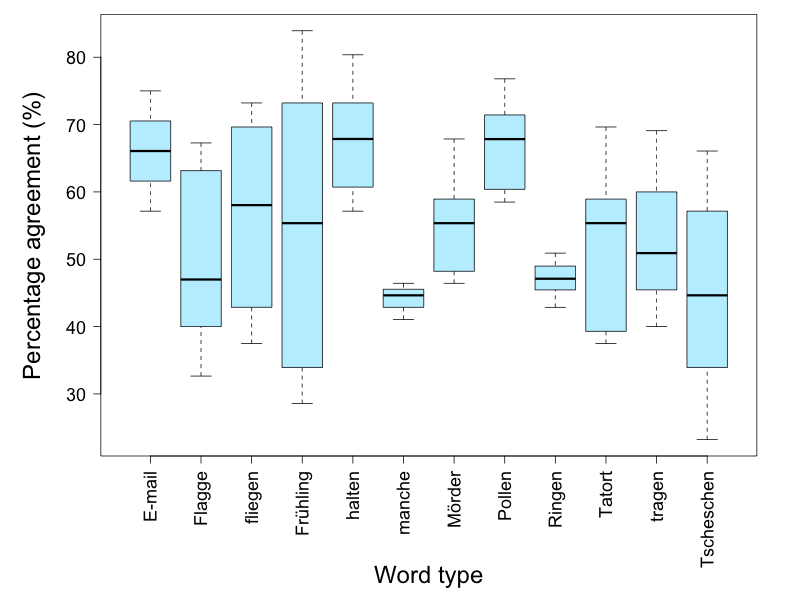
\includegraphics[width=.9\textwidth]{img/plots/pairwisePctByWord-noTitle}
				\label{fig:agreement:words:pct}
			\end{subfigure}%
			
			\vspace{2em}
			
			\begin{subfigure}{\textwidth}
				\centering
				\caption{Pairwise $\kappa$ by word type}
				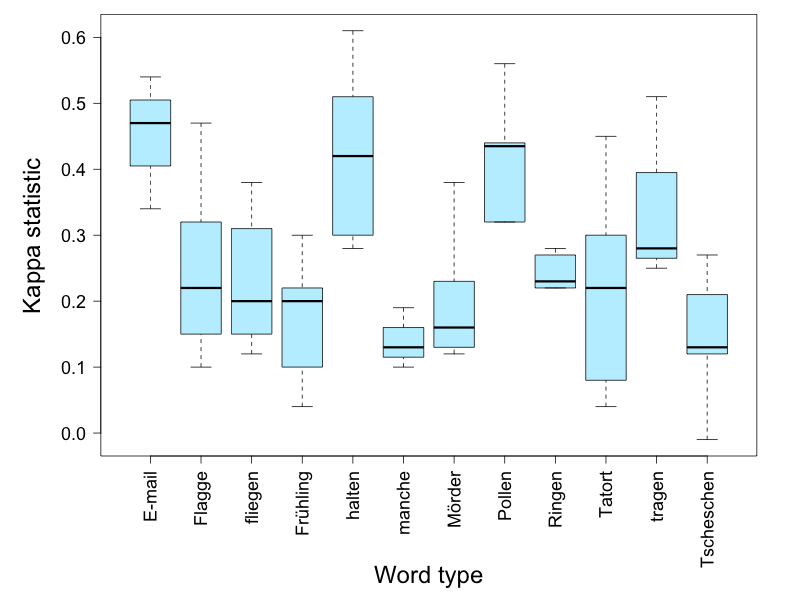
\includegraphics[width=.9\textwidth]{img/plots/pairwiseKappaByWord-noTitle}
				\label{fig:agreement:words:k}
			\end{subfigure}%
			
			\vspace{1em}	
			
			
			\caption[Pairwise agreement statistics by word type]{Pairwise agreement between annotators for each word type. 	
			Horizontal lines represent median values. Colored boxes extend from the first quartile to the third quartile, and thus represent the Inter Quartile Range (IQR). Whiskers extend to the minimum and maximum values within 1.58 IQR of the first and third quartiles, respectively, and roughly represent a 95\% confidence interval around the median. 
			 Outliers that fall outside of the IQR by a distance of more than approximately 1.5$\times$IQR  are represented by circles.
			%Numbers in parentheses indicate the number of pairwise comparisons available for each word type. The bottom of each vertical bar represents the minimum pairwise value, the top the maximum. Horizontal bars indicate average pairwise values.
			}

			
			
			\label{fig:agreement:words}
		\end{figure}
		
		
		
		
	To put these agreement values in context, it is worthwhile to compare them with those obtained in recent work by \textcite{Michaux2013} on L2 Dutch speech by L1 French speakers. In this study, three expert annotators were asked to indicate the syllable they perceived as stressed in Dutch word utterances by the L1 French speakers. Two of the annotators were L1 Dutch speakers, the other an L1 French speaker who was nevertheless ``highly proficient'' in Dutch (p.~90). The authors report an average $\kappa$ of 0.71 between annotators, representing ``substantial'' agreement in the schema of \textcite{Landis1977}, and a much higher value than those observed in the present work. One plausible explanation for this difference may be the fact that while the three annotators participating in the \textcite{Michaux2013} study were all ``phonetically trained'' (p.~90), i.e. experts (see \cref{sec:lexstress:annotators}),
	the annotation project described here collected judgments from a larger number of annotators, and only two of the 15 participating annotators had extensive phonetic training. The relationship between annotator expertise and inter-annotator agreement is explored further in \cref{sec:agreement:expert}. 
		
			The following sections present detailed analyses of the agreement between annotators with different native languages (\cref{sec:agreement:native}) and different levels of expertise (\cref{sec:agreement:expert}).  However, on the whole, it already seems evident that inter-annotator agreement in this lexical stress error annotation task is relatively low. This may simply signal low reliability among the particular annotators participating in this study, but it may also be a preliminary indication of the considerable difficulty of the task of diagnosing errors in L1 French speakers' realizations of lexical stress in German; this notion will be revisited in \cref{sec:diag:classification}. 

	
	
		%\subsubsection{Native vs. nonnative annotators}
		%\subsection{Native vs. nonnative annotators}
		\subsection{Native vs. nonnative annotators}
		\label{sec:agreement:native}

		
		
		Going beyond the coarse-grained analysis of inter-annotator agreement described in the previous section, we come now to the second question raised at the beginning of this chapter:
		
		\textit{Are there differences in how native and nonnative German speakers identify errors?}
		
		%\TODO{expectations/speculations of what we will find?}
		
		To answer this question, it is useful to look at the inter-annotator agreement between native and nonnative annotators, as well as at the distribution of label types within each group. 
		
		\Cref{fig:agreement:L1} illustrates the inter-annotator agreement for all pairs in which one annotator was a native German speaker and the other a nonnative speaker, as well as agreement between pairs in which both annotators were native speakers. Due to the small size of the nonnative group (3 annotators) and the aforementioned technical problems with annotator G's data (see \cref{sec:lexstress:annotators}), there was very little overlap between nonnative annotators (only one pairwise comparison), preventing meaningful analysis of agreement within the nonnative group. The precise mean, maximum, median, and minimum pairwise values for the two agreement metrics are listed in \cref{tab:agreement:L1}, for both  native-nonnative pairs and native-native pairs. 
		
		Looking at these statistics, we see little difference between the two types of pairs; in particular, the mean percentage agreement and $\kappa$ values for native-nonnative and native-native pairs are quite close. If anything, it would appear that agreement within the native annotator group is slightly lower and more varied than agreement between the native and nonnative groups, though this may be explained by the larger number of native-native pairs compared to native-nonnative. It would therefore seem that these inter-annotator statistics do not tell us much about difference between how the two groups of annotators judge lexical stress accuracy.
		
		
		\begin{table}[tb]
			\centering
			\caption{Inter-annotator agreement between native and nonnative annotators (pairwise)}
			%\begin{tabularr}{\textwidth}{lXXXX}
			\begin{tabular}{lrrrr}
			\toprule
			& \multicolumn{2}{c}{Native vs. nonnative} & \multicolumn{2}{c}{Native vs. native} \\
			\cmidrule(lr){2-3} \cmidrule(lr){4-5}
			& \% Agreement & Cohen's $\kappa$ & \% Agreement & Cohen's $\kappa$  \\
			\midrule
Mean	&56.98\%	 & 0.29  & 53.87\%	& 0.25\\
Maximum&	76.79\%	& 0.56 & 83.93\%	 & 0.61\\
Median	& 57.14\%	 &0.25 &  50.91\%	& 0.23 \\
Minimum	&32.65\%	 & 0.10 &  23.21\% &	-0.01\\
			\bottomrule
			\end{tabular}
			\label{tab:agreement:L1}
		\end{table} 
		
		\begin{figure}[h!]
			\centering
			
%			\begin{subfigure}[b]{.5\textwidth}
%				\centering
%				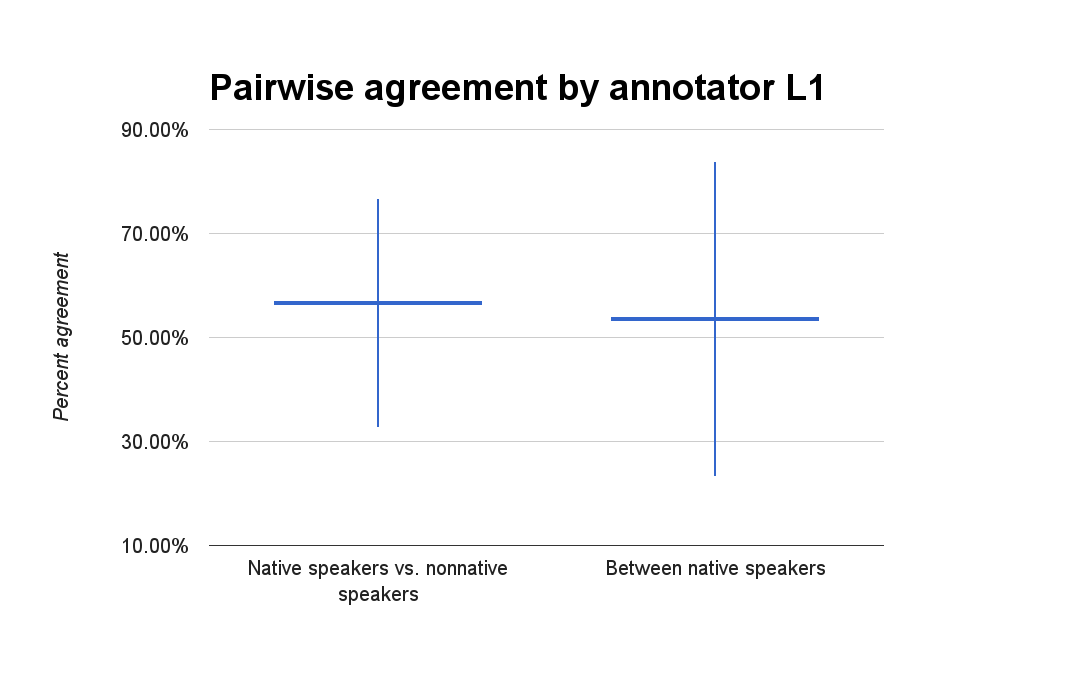
\includegraphics[width=\textwidth]{img/annotation/pairAgreeL1}
%				\caption{Percent agreement}
%				\label{fig:agreement:L1:pct}
%			\end{subfigure}%
%			~
%			\begin{subfigure}[b]{.5\textwidth}
%				\centering
%				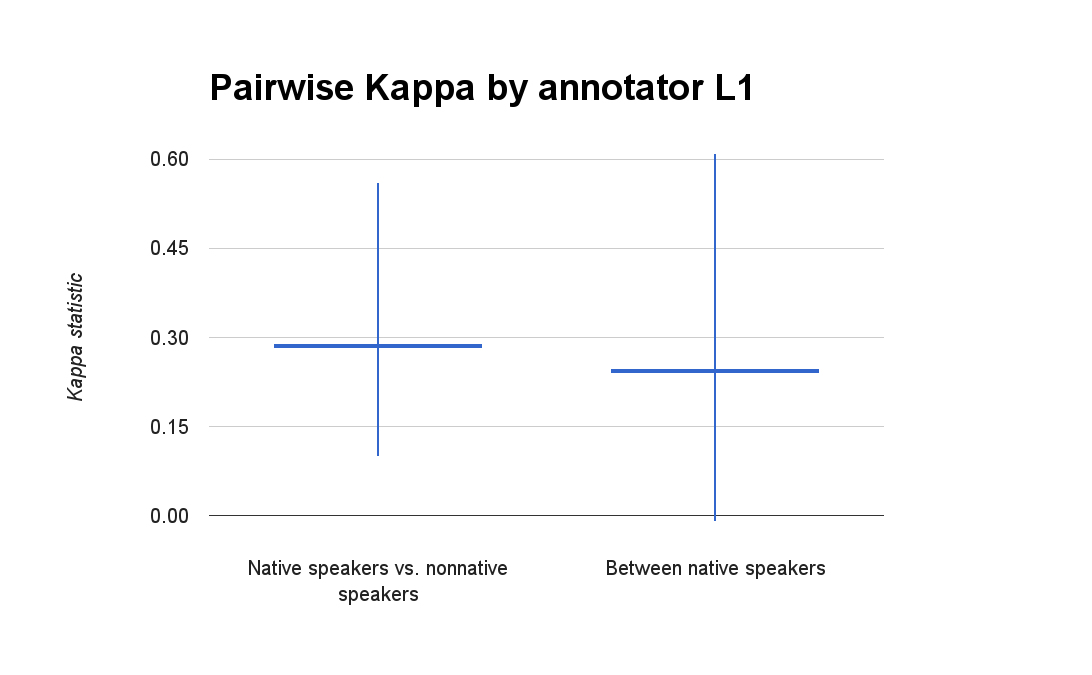
\includegraphics[width=\textwidth]{img/annotation/pairKappaL1}
%				\caption{Cohen's Kappa statistic}
%				\label{fig:agreement:L1:k}
%			\end{subfigure}%
			
			\begin{subfigure}{.5\textwidth}
				\centering
				\caption{Pairwise \% agreement by L1 group}
				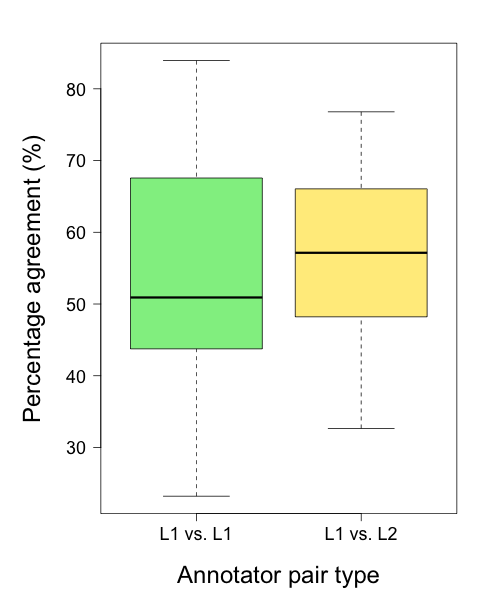
\includegraphics[width=\textwidth]{img/plots/pairwisePctByL1-noTitle}
				\label{fig:agreement:L1:pct}
			\end{subfigure}%
			~
			\begin{subfigure}{.5\textwidth}
				\centering
				\caption{Pairwise $\kappa$ by L1 group}
				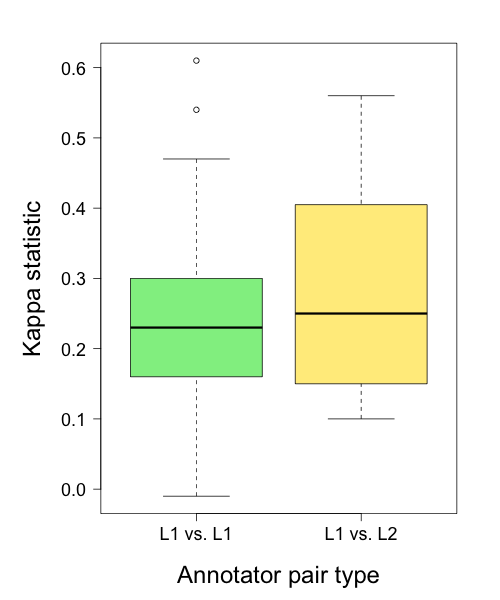
\includegraphics[width=\textwidth]{img/plots/pairwiseKappaByL1-noTitle}
				\label{fig:agreement:L1:k}
			\end{subfigure}%
			
			\caption[Pairwise agreement statistics by annotator L1 group]{\TODO{larger labels?} Pairwise agreement between annotators based on L1 group (L1 = native German speaker, L2 = nonnative speaker). 
			Horizontal lines represent median values. Colored boxes extend from the first quartile to the third quartile, and thus represent the Inter Quartile Range (IQR). Whiskers extend to the minimum and maximum values within 1.58 IQR of the first and third quartiles, respectively, and roughly represent a 95\% confidence interval around the median. 
			 Outliers that fall outside of the IQR by a distance of more than approximately 1.5$\times$IQR  are represented by circles.
			%The bottom of each vertical bar represents the minimum pairwise value, the top the maximum. Horizontal bars indicate average pairwise values.
			}
			\label{fig:agreement:L1}
		\end{figure}
		
		

		However, in comparing the relative frequencies of the different labels assigned by annotators in these two L1 groups, a more noticeable difference between the groups begin to emerge. As illustrated in \cref{fig:agreement:l1bars}, the native and nonnative speakers judged utterances as having correct lexical stress with approximately the same frequency: 52.7\% of native annotators' judgments were [correct], vs. 57.3\% for nonnative annotators. However, nonnative speakers seemed to choose the [none]
		%``no clear stress/I can't tell'' 
		label somewhat more frequently than native speakers (21.3\% vs. 11\%); this could indicate that nonnative speakers are less confident about how stress should be realized in German, resulting in less certainty about whether a given utterance is correct or not. \TODO{update/verify this paragraph}
		
		
			\begin{figure}[htb]
				\centering
				\caption[Distribution of labels by annotator L1]{Distribution of labels assigned by native and nonnative annotators,
				as a percentage of the total number of utterances labeled by that annotator group \TODO{add exact values?}
				}
				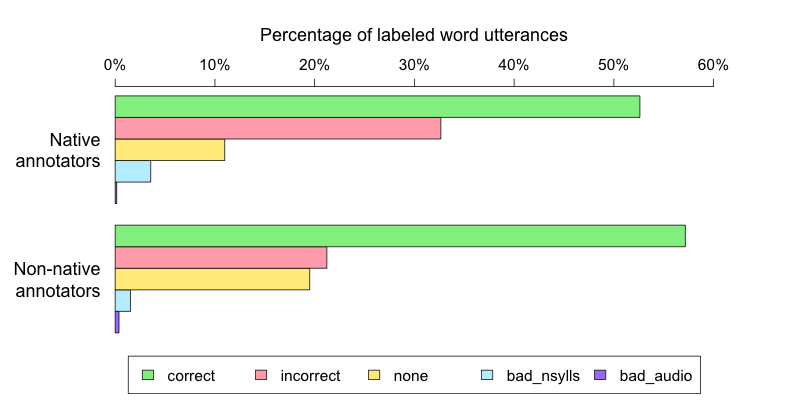
\includegraphics[width=\textwidth]{img/plots/pctJudgmentsByL1-notStacked}
				\label{fig:agreement:l1bars}
			\end{figure}
			
%			\begin{figure}[htb]
%				\centering
%				\caption{Stress judgments by native and nonnative annotators}
%				\includegraphics[width=.9\textwidth]{img/plots/pctJudgmentsByL1-NoTitle}
%				\label{fig:agreement:l1bars}
%			\end{figure}
	
%			\begin{figure}[htb]
%				\centering
%				\begin{subfigure}[b]{.5\textwidth}
%					\centering
%					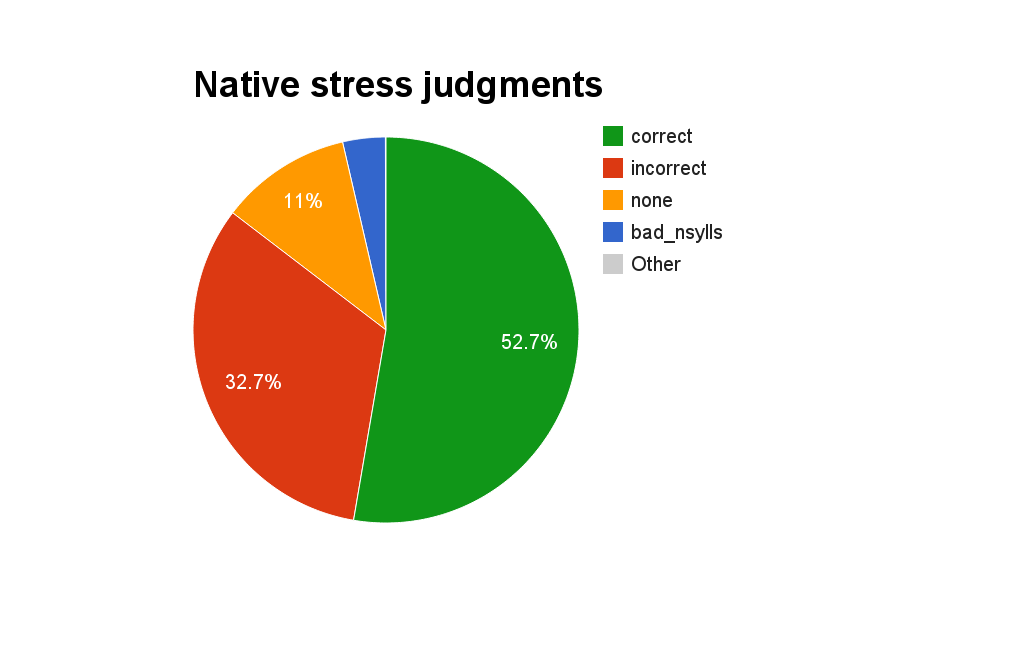
\includegraphics[width=\textwidth]{img/annotation/nativePie}
%					\caption{Native annotators}
%					\label{fig:l1pies:native}
%				\end{subfigure}%
%				~
%				\begin{subfigure}[b]{.5\textwidth}
%					\centering
%					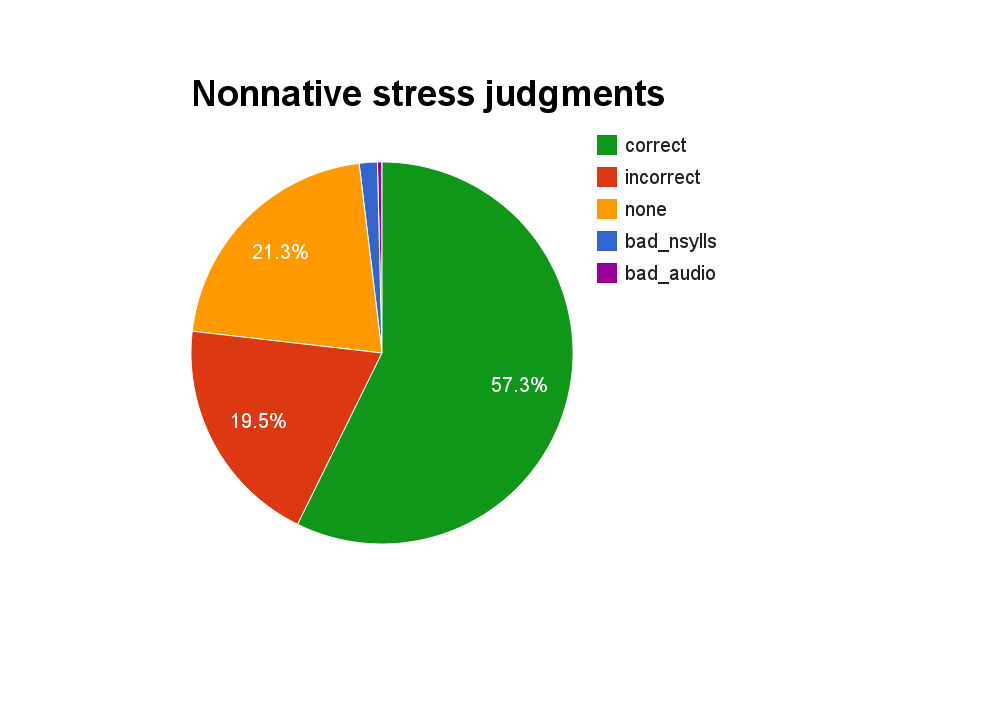
\includegraphics[width=\textwidth]{img/annotation/nonnativePie}
%					\caption{Nonnative annotators}
%					\label{fig:l1pies:nonnative}
%				\end{subfigure}%
%				\caption{Stress judgments made by native and nonnative German speakers}
%				\label{fig:l1pies}
%			\end{figure}
			
		Though the differences between native and nonnative annotators are interesting from the perspective of L2 perception of lexical stress, the ultimate goal of this thesis project is to create a CAPT tool which will help L1 French speakers be more intelligible when speaking German as L2, and therefore the way in which native German speakers perceive lexical stress in nonnative speech is of more relevance to this work than the way it is perceived by nonnative speakers. Therefore, the remainder of this chapter is concerned exclusively with the judgments of native annotators, which is to say that judgments by nonnative annotators are not included in the analyses that follow.
			
		
		\subsection{Expert vs. intermediate vs. novice annotators}
		\label{sec:agreement:expert}
		
		
		
	This section brings us to the last of the questions raised at the beginning of the chapter concerning inter-annotator agreement in the stress-annotated data, namely:
	
	\textit{Are there differences in how 
	%expert and novice annotators 
	annotators with different levels of expertise
	identify lexical stress errors?}
	
	Given the general difficulty of the task of identifying lexical stress errors, evidenced by relatively low overall inter-annotator agreement as discussed in \cref{sec:agreement:overall} above, it might seem reasonable to suppose that training in phonetics/phonology or experience annotating (nonnative) speech might have a positive impact on an annotator's ability to reliably judge the accuracy of lexical stress realizations by nonnative speakers. However, it once again bears mentioning that the ultimate goal of this work is to help L2 learners communicate intelligibly in German, and it can safely be assumed that in the vast majority of cases such learners will be communicating more often with native speakers who possess little formal knowledge of speech science than with expert phoneticians. Therefore, even if differences in reliability do exist between expert and novice annotators, it is important that the perception of nonnative lexical stress errors by non-experts not be ignored in favor of perception of such errors by experts. 
	
	%\TODO{mention that we're trying to train nonnative speakers to communicate in the L2, which means their speech will be ``evaluated'' by novices (native speakers), so we don't want to limit ourselves to expert judgments}

	\TODO{Better transition needed here?}
	
	Just as the previous section analyzed native vs. nonnative annotations in terms of inter-annotator agreement and differences in label distributions between those groups, this section uses analogous data to investigate the differences between annotators of the three different expertise levels -- expert (exp.), intermediate (int.), and novice (nov.) -- described in \cref{sec:lexstress:annotators} above.
	
	To determine inter-annotator agreement between the three expertise groups, percentage agreement and $\kappa$ were tabulated for each pairing of annotators from different groups, i.e. for each of the following three pair types:
	
	\begin{itemize}
	\item{Expert annotator vs. novice annotator}
	\item{Expert annotator vs. intermediate annotator}
	\item{Novice annotator vs. intermediate annotator}
	\end{itemize}
	
	Additionally, pairwise agreement was tallied for pairings between two intermediate annotators, as a measure of inter-annotator agreement within this expertise group. Due to the small size of the expert and novice groups (two and three annotators, respectively), as well as the fact that expert annotators were deliberately not assigned overlapping tokens to label in an effort to maximize the number of tokens labeled by at least one expert \TODO{does that contradict the above statement about novice judgments being just as important as expert ones?}, overlap within these groups was insufficient to calculate meaningful intra-group agreement statistics, so none are reported here. The small size of these two groups should also be kept in mind throughout the following analysis, as we should hesitate to draw firm conclusions from such small samples. 
		
		The agreement measures between groups and within the intermediate group are presented in \cref{tab:agreement:expertise} and illustrated in \cref{fig:agreement:expertise}. As these figures show, the mean values of both percentage agreement and $\kappa$ between the different expertise groups are quite close, and close to the overall means for all annotator pairs;  interestingly, the highest mean percentage agreement observed in this comparison (though only by a small margin) is that of expert-novice pairings, which might be a preliminary indication that there is no relevant difference in reliability between expertise levels. 
			
		
		
		\begin{table}[tb]
			\centering
			\caption[Pairwise agreement statistics by annotator expertise]{Pairwise agreement between annotators based on their level of expertise: expert (Exp), intermediate (Int), or novice (Nov).
			%{Pairwise agreement between expertise groups \TODO{explain abbreviations}
			}
			\begin{tabularx}{\textwidth}{lXXXXXXXX}
				\toprule
		& \multicolumn{2}{c}{Exp vs. Nov} & \multicolumn{2}{c}{Exp vs. Int} & \multicolumn{2}{c}{Nov vs. Int} & \multicolumn{2}{c}{Int vs. Int} \\
	&\% Agr.	& $\kappa$	&\% agr. &	$\kappa$&	\% agr.	& $\kappa$	&\% agr. & $\kappa$ \\
	\midrule
Mean	& 57.89\%	& 0.23	& 55.30\%	& 0.23	& 52.12\%	& 0.26	& 51.44\%	& 0.23 \\
Maximum	& 71.43\%	& 0.44	& 83.93\%	& 0.32	& 71.43\% & 	0.47	& 80.36\%	& 0.61 \\
Median	& 68.46\%	& 0.24	& 49.95\%	& 0.25	& 51.70\%	& 0.26	& 47.58\%	& 0.22\\
Minimum	& 23.21\%	& -0.01	& 33.93\%	& 0.10	& 35.71\%	& 0.08	& 28.57\%	&  0.04 \\
				\bottomrule
			\end{tabularx}
			\label{tab:agreement:expertise}
		\end{table}
			
		
		
		\begin{figure}[p]
			\centering
			
%			\begin{subfigure}[b]{.5\textwidth}
%				\centering
%				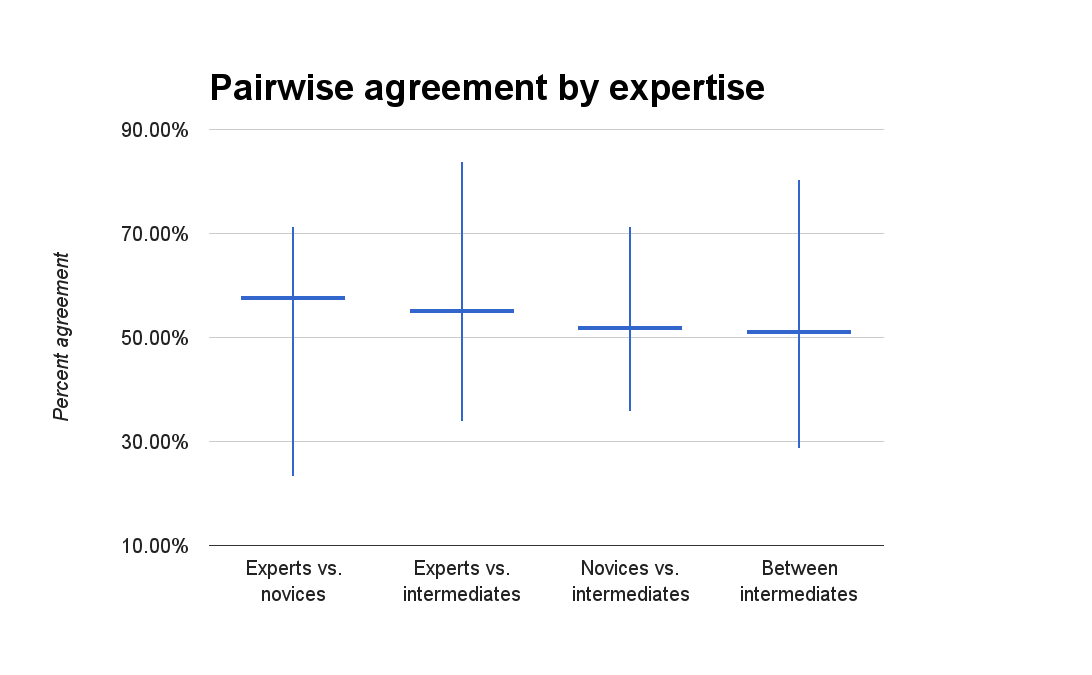
\includegraphics[width=\textwidth]{img/annotation/pairAgreeExpertise}
%				\caption{Percent agreement}
%				\label{fig:agreement:expertise:pct}
%			\end{subfigure}%
%			~
%			\begin{subfigure}[b]{.5\textwidth}
%				\centering
%				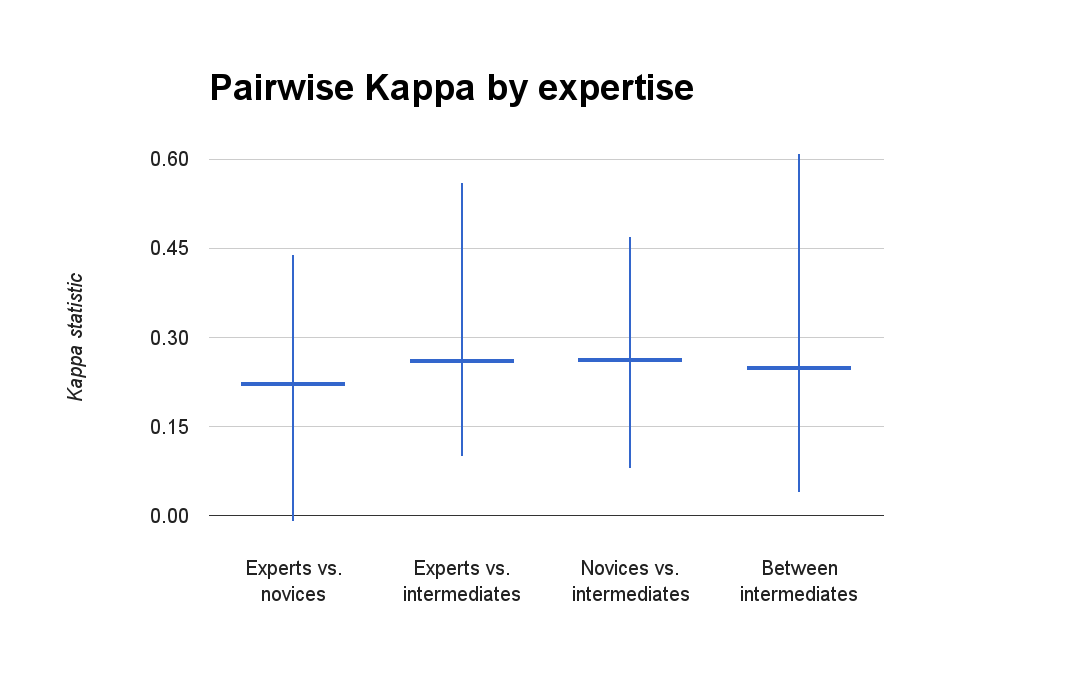
\includegraphics[width=\textwidth]{img/annotation/pairKappaExpertise}
%				\caption{Cohen's Kappa statistic}
%				\label{fig:agreement:expertise:k}
%			\end{subfigure}%
			
			\begin{subfigure}{\textwidth}
				\centering
				\caption{Pairwise \% agreement by expertise group}
				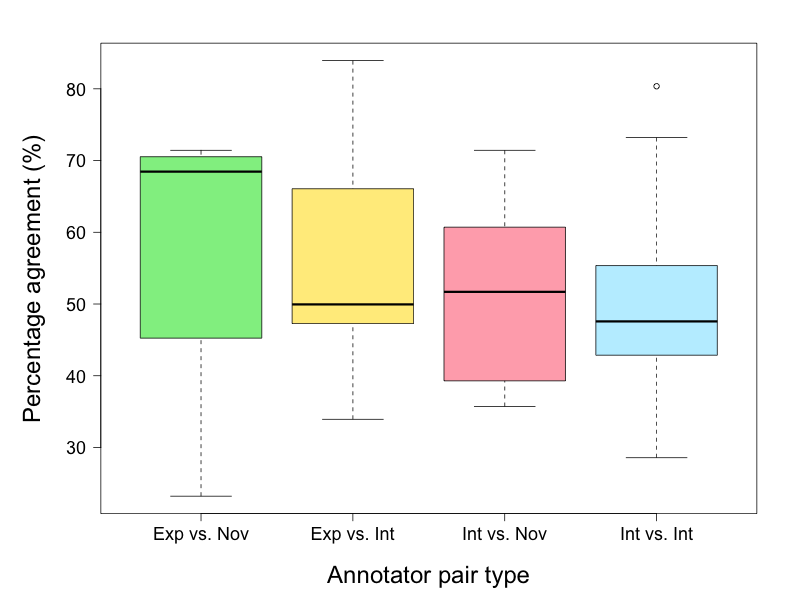
\includegraphics[width=.9\textwidth]{img/plots/pairwisePctByExpertise-noTitle}
				\label{fig:agreement:expertise:pct}
			\end{subfigure}%
			
			\vspace{1em}			
			
			\begin{subfigure}{\textwidth}
				\centering
				\caption{Pairwise $\kappa$ by expertise group}
				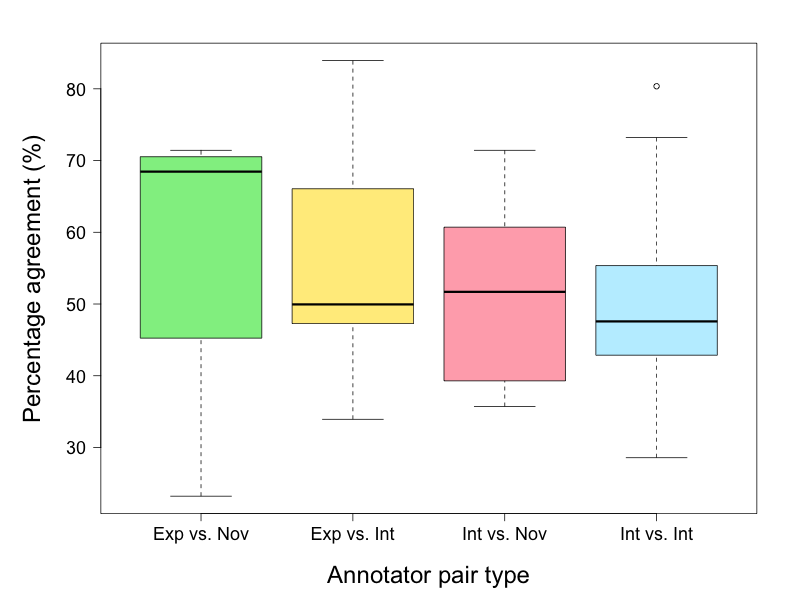
\includegraphics[width=.9\textwidth]{img/plots/pairwisePctByExpertise-noTitle}
				\label{fig:agreement:expertise:k}
			\end{subfigure}%
			
			\caption[Pairwise agreement statistics by annotator expertise]{Pairwise agreement between annotators based on their level of expertise: expert (Exp), intermediate (Int), or novice (Nov). 
			\TODO{boxplot description}
			%The bottom of each vertical bar represents the minimum pairwise value, the top the maximum. Horizontal bars indicate average pairwise values.
			}
			\label{fig:agreement:expertise}
		\end{figure}
		
			\Cref{fig:agreement:expertisebars} illustrates the relative number of each label type as assigned by annotators of the three expertise levels described in \cref{sec:lexstress:annotators} above, and while any analysis of this data should bear in mind the small sample sizes of the expert and novice groups (two and three annotators, respectively), it does appear that some interesting differences may exist between the three groups. 
			
			Expert annotators seem to be far more ``generous'' in their labeling than intermediate or novice annotators, in that the experts assigned the [correct] label 73.6\% of the time, in contrast with 49.3\% and 54.8\% for the other two groups respectively. One could speculate that experts' familiarity with nonnative speech and knowledge of possible inter-speaker variations in lexical stress realization may be the cause for this willingness to accept a high proportion of utterances as correct. 
			
			Another interesting difference can be observed between the intermediate and novice annotator groups: compared with the intermediate annotators, novices assign the [none] label less frequently (5.8\% of the time, versus 16.3\% for intermediates) and the [bad\_nsylls] label more frequently (8.4\% of the time, versus 2.1\% for intermediates). Still keeping in mind the discrepancy in sample sizes when comparing 10 intermediate annotators to three novices, 
			%\TODO{we might} speculate
			it seems plausible that if experts' extensive experience with nonnative speech could be an explanation for their aforementioned ``generosity'' with the [correct] label, novice annotators' lack of experience with nonnative speech could in a similar way make them ``harsher'' in judging nonnative utterances as having an incorrect number of syllables. 
			
			\begin{figure}[tb]
				\centering
				\caption[Distribution of labels by annotator expertise]{Distribution of labels assigned by annotators of different expertise levels,
				as a percentage of the total number of utterances labeled by that annotator group
				}
				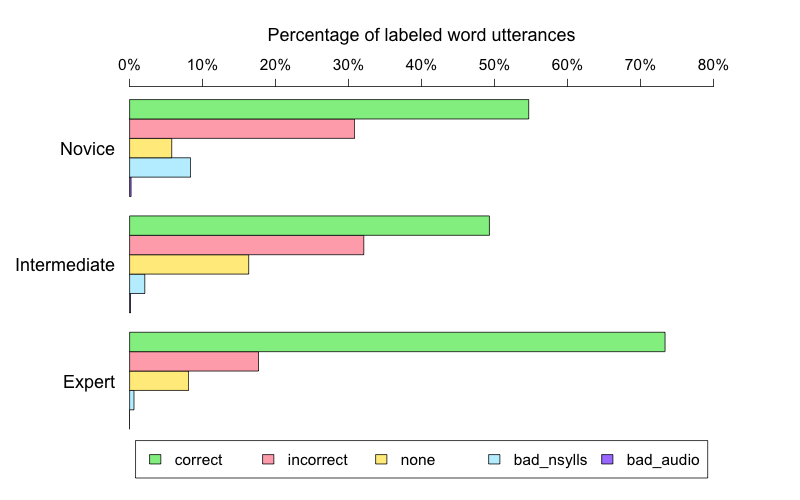
\includegraphics[width=\textwidth]{img/plots/pctJudgmentsByExpertise-notStacked}
				\label{fig:agreement:expertisebars}
			\end{figure}			
			
			
%			\begin{figure}[htb]
%				\centering
%				\caption{Stress judgments by annotator expertise}
%				\includegraphics[width=.9\textwidth]{img/plots/pctJudgmentsByExpertise-NoTitle}
%				\label{fig:agreement:expertisebars}
%			\end{figure}
			
%			\begin{figure}[htb]
%				\centering
%				\begin{subfigure}[b]{.5\textwidth}
%					\centering
%					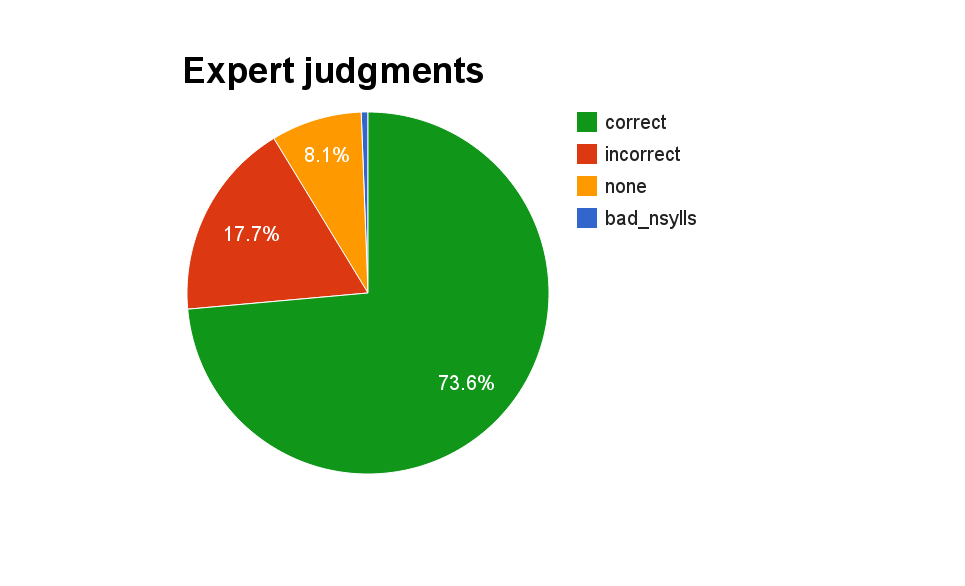
\includegraphics[width=\textwidth]{img/annotation/expertPie}
%					\caption{Expert}
%					\label{fig:expertisepies:expert}
%				\end{subfigure}%
%				
%				\begin{subfigure}[b]{.5\textwidth}
%					\centering
%					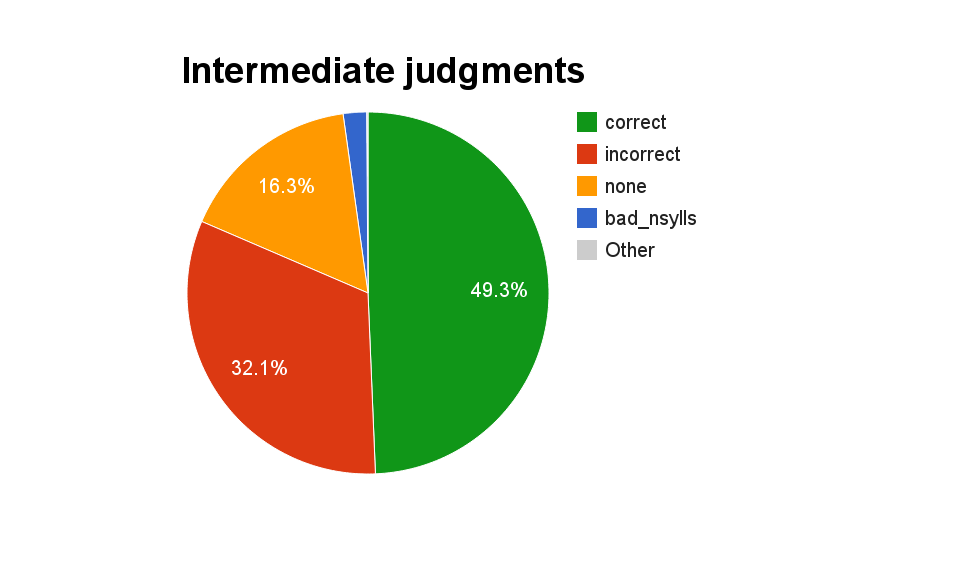
\includegraphics[width=\textwidth]{img/annotation/intermediatePie}
%					\caption{Intermediate}
%					\label{fig:expertisepies:intermediate}
%				\end{subfigure}%
%				~
%				\begin{subfigure}[b]{.5\textwidth}
%					\centering
%					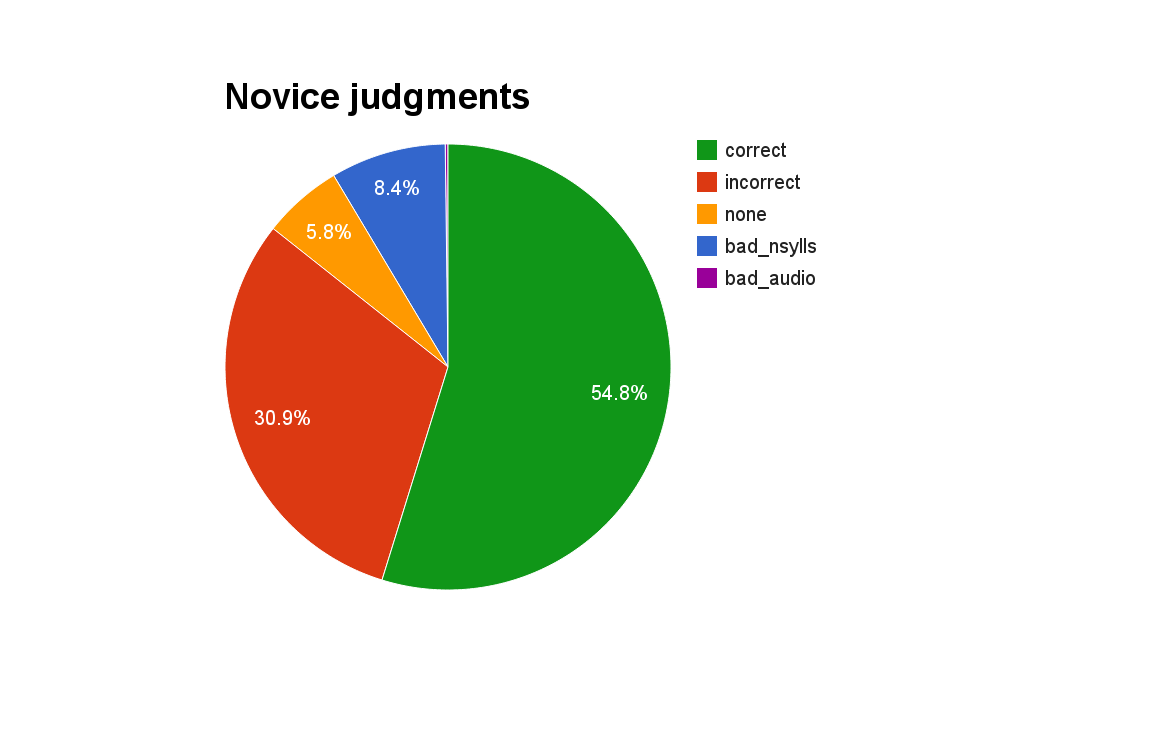
\includegraphics[width=\textwidth]{img/annotation/novicePie}
%					\caption{Novice}
%					\label{fig:expertisepies:novice}
%				\end{subfigure}%
%				\caption{Stress judgments by annotator expertise}
%				\label{fig:expertisepies}
%			\end{figure}
			
			
			
		\section{Choosing gold-standard labels}
		\label{sec:agreement:gold}
		
		\TODO{Check for errors related to re-sectioning}
		
		
		As the previous sections have illustrated, having multiple annotators judge the accuracy of each lexical stress production was useful insofar as it led to some interesting observations about the difficulty of reliably assessing lexical stress accuracy, as well as insight into the differences in how judgments by annotators with different native languages and levels of expertise compare. However, if the annotations are to be used for \TODO{training an automated error-diagnosis system}, each token in the sub-corpus must ultimately be assigned a single ``gold-standard'' label from the set of possible labels described in \cref{sec:lexstress:method}.
		% which will be referred to henceforth as  $S$: $\{$[correct],{[incorrect]},{[none]},{[bad\_nyslls]},{[bad\_audio]}$\}$. 
		
		In some cases, this assignment was trivial, while in others a decision had to be made between competing candidate labels. This section describes the procedure by which a single gold standard label was chosen for each word token (utterance) in the data set described in \cref{sec:lexstress:data}. In the remainder of this section, the gold-standard label chosen for a given word token $t$ will be referred to as $s_{\text{gold}}(t)$, where $s \in S = \{$[correct],{[incorrect]},{[none]},{[bad\_nyslls]},{[bad\_audio]}$\}$ stands for one of the possible labels.
		
		To prepare for gold-standard labeling, all available annotations for $t$ were tallied by their label type $s$, resulting in a set $S_t \subseteq S$ of labels assigned to $t$ by any of the native annotators who labeled this token (nonnative annotators' judgments were omitted as mentioned in \cref{sec:agreement:native} above). For each label $s(t) \in S_t$, the number of ``votes'' for that label was recorded as the number of annotators who assigned this label to token $t$; henceforth \TODO{\textit{need better notation for maxvotes set: }$S_{\text{max}} \subseteq S_t$} will refer to the set of labels for $t$ with the highest number of votes \TODO{reword?}.
		
		Given the observed labels and their vote counts, a rule-based procedure was followed to assign a gold-standard label $s_{\text{gold}}(t)$ to each token $t$ in the annotated sub-corpus; this procedure is outlined in \cref{tab:agreement:goldrules}. At each step $i$ in the procedure, any tokens whose set $S_t$ of observed labels fits condition $C_i$ are assigned the gold-standard label described in column $s_{\text{gold}}(t)$; the number of tokens matching $C_i$ is given as $N(C_i)$, and 
		% gives the number of tokens labeled at this step, i.e. the number matching $C_i$. The rightmost column 
		$N(C_{1 \dots i})$ represents the total number of tokens which have been assigned a gold-standard label at the end of step $i$ in the labeling procedure (i.e. the number of tokens matching $C_i$ or any previous condition).
		
		

		\begin{table}[htb]
		\caption[Procedure for choosing a gold-standard label for a given token]{Procedure for choosing a gold-standard label $s_{\text{gold}}(t)$ for a given token $t$. At step $i$, tokens matching $C_i$ are assigned the label in column $s_{\text{gold}}(t)$. The rightmost columns $N(C_i)$ and $N(C_{1 \dots i})$ list the number of tokens labeled in step $i$ and the total number that have been labeled at the end of step $i$, respectively.}
			\begin{tabularx}{\textwidth}{rXlrr}
			\toprule
			Step ($i$)
			& Condition ($C_i$) \TODO{reword w/ $S_t$\&$S_{\text{max}}$} & $s_{\text{gold}}(t)$ & $N(C_i)$ & $N(C_{1 \dots i})$ \\
			\midrule
			
			1.& There is only one label $s_{\text{only}}$ with any votes & 
			%$s_{\text{gold}}(t) \gets 
			$s_{\text{only}}$ & 268 & 268 \\
			 
			2.& One label $s_{\text{max}}$ has more votes than any other labels & 
			%$s_{\text{gold}}(t) \gets 
			$s_{\text{max}}$ & 265 & 533 \\
			
			3.& There is a label $s_{\text{expert}}$ assigned by an expert & 
			%$s_{\text{gold}}(t) \gets 
			$s_{\text{expert}}$ & 51 & 584 \\
			
			4.& \mbox{[bad\_nsylls]} is one of the competing labels, 
			%ignore it; \newline if 
			and there is only one other competing label $s_{\text{only}}$  \TODO{reword}
			%remains 
			& 
			%$s_{\text{gold}}(t) \gets 
			$s_{\text{only}}$ & 17 & 601 \\
			
			5.& There is a three-way tie between labels
			%, indicating that the accuracy of the lexical stress realization is not clear 
			&
			% [correct], [none], and [incorrect] & 
			%$s_{\text{gold}}(t) \gets$ 
			\mbox{[none]} & 6 & 607\\
			
			6.& There are two competing labels: 
			%one of which is 
			\mbox{[none]} and 
			%the other of which is 
			$s_{\text{certain}} \in \{$[correct],[incorrect]$\}$ &
			$s_{\text{certain}}$ & 21 & 628\\
			
			7.& There are two competing labels: \mbox{[correct]} and \mbox{[incorrect]} &
			\mbox{[correct]} & 40 & 668\\
	
			\bottomrule
			\end{tabularx}
		\label{tab:agreement:goldrules}
		\end{table}
		
				
		
		
		\TODO{Check following paragraphs for consistency of terms - shouldn't "Condition 1" be $C_1$, etc.?}
		
		As mentioned in \cref{sec:agreement:overall}, for 268 of the 
		%669 
		668 tokens annotated, there was no disagreement whatsoever between annotators: for each of these 268 tokens, all annotators who labeled the token made the same judgment, making it easy to assign this label as the gold standard for this utterance. Condition 1 in \cref{tab:agreement:goldrules} captures this category of tokens. 
		%
		For another 265 tokens, a majority of annotators assigned the same label, though one or more annotators dissented, so assigning the majority-vote label as the gold standard is logical; these are captured by Condition 2 \TODO{$C_2$?} in the table. Therefore, for a total of 533 tokens (approximately 80\% of the word utterances in the sub-corpus), the choice of $s_{\text{gold}}(t)$ was uncontroversial.
		
		For the remaining 
		%116 
		utterances, choosing gold-standard labels was a less straightforward task,
		and the decisions made in steps 3-7 are somewhat more controversial.
		%3
		%In a third step, i
		If either of the two expert annotators had labeled one of the remaining tokens, the expert's judgment was taken as the gold standard; 51 tokens met this condition ($C_3$). 
		%4
		Next, in step 4, if there were exactly two labels in $S_{\text{max}}$ and one of them was [bad\_nsylls], the other label was chosen as $s_{\text{gold}}(t)$. The reasoning behind this step is that since the label [bad\_nsylls] was intended to be applied to utterances for which no stress judgment was possible, then if at least one annotator was able to make a judgment, the [bad\_nsylls] label must not be appropriate and should be rejected. This condition ($C_4$) applied to 17 tokens. 
		%5
		The following step (5) addressed tokens for which the set of competing labels $S_{\text{max}}$ had three members, i.e. for which there was a three-way tie between labels. The fact that so many different labels were assigned to each of these tokens was taken as an indication that the accuracy of the lexical stress realization in this utterance was quite difficult to judge, i.e. it is unclear which syllable in the uttered word has been stressed; as the label [none] is intended to capture such cases, this label was chosen as the gold standard for the 6 utterances matching this condition ($C_5$).
		%6
		The next condition ($C_6$) captured the 21 cases in which $S_{\text{max}}$ contained exactly two labels competing for gold-standard status, with one of the labels being [none] and the other being one of the two labels associated with certainty about the accuracy of the lexical stress realization, i.e. [correct] or [incorrect]. In these cases, [none] was rejected in favor of the certain label, based on the assumption that if at least one annotator was able to categorically classify the given utterance as correct or incorrect in terms of lexical stress, other native-speaking listeners might be inclined to make the same judgment \TODO{fix that sentence}.
		%7
		The remaining 40 utterances were captured by the seventh and final condition, $C_7$, in which $S_{\text{max}}$ contained exactly two labels: [correct] and [incorrect]. In these cases, the learner's utterance was assessed generously and the [correct] label was chosen as $s_{\text{gold}}(t)$, to capture the fact that as mentioned in \cref{sec:agreement:overall}, assessing the accuracy of a lexical stress realization seems to be a somewhat difficult task, and if at least one of the native speakers who heard the given utterance were willing to accept its stress realization as correct, the learner should not be \TODO{``penalized''} by an [incorrect] label.
		
		Despite the necessarily controversial nature of some of the labeling decisions described above, in the remainder of this thesis, the gold-standard labels chosen thus are taken as the ground truth for the distribution of lexical stress errors in this annotated subset of  668 word utterances from the IFCASL corpus. These gold-standard labels are used to analyze the distribution of errors in the corpus (see the following section), and also serve as training data for the supervised machine learning approach to stress error diagnosis described in  \cref{chap:diagnosis}\TODO{more specific section reference}. 
		
		
		%%%%	ORIGINAL RULES (BEFORE 6.3.15)
%%%%		Original rules:
%%%%		\begin{itemize}
%%%%		\item{if there is only one label or a majority vote, use that}
%%%%		\item{if one of the annotators is an expert (FZ, JJ, or RM), use that}
%%%%		\item{if [bad\_nsylls] is one of the best labels, ignore it}
%%%%		\item{if it was judged both correct and incorrect (i.e. both [correct] and [incorrect] are in the best labels), choose [none]}
%%%%		\item{if there are two best labels and one is [none], choose the more certain label (i.e. ignore [none])}
%%%%		\end{itemize}
%%%%		
%%%%		\begin{tabular}{ll}
%%%%				Original breakdown:\\
%%%%		ignore\_none &	 19 \\
%%%%ignore\_badsylls &	 0\\
%%%%no\_decision &	 0\\
%%%%incorrect+correct=none &	 36\\
%%%%single\_label &	 268\\
%%%%majority\_vote (533 - 268) &	 265\\
%%%%expert\_wins &	 81\\
%%%%		\end{tabular}
	
%%%%	RESULTS USING NEW RULES:		
%%%%	rejected :	 1
%%%%	threeway :	 6
%%%%	incorrect+none+correct=none :	 0
%%%%	expert_wins :	 51
%%%%	value_certainty :	 21
%%%%	ignore_none :	 0
%%%%	ignore_badsylls :	 17
%%%%	generosity :	 40
%%%%	ignore_badwords :	 0
%%%%	single_label :	 268
%%%%	majority_vote_or_single :	 533
%%%%	no_decision :	 0
%%%%	
%%%%	Rejected due to disfluencies:
%%%%	('2SR31_FGBA2_547', 'tatort')
		
%		\begin{algorithm}[h!]
%			\caption*{Procedure for choosing a gold-standard label  for a given token ($s_{\text{gold}}(t)$)}
%			\begin{algorithmic}
%				%\State $T \gets $ the set of word tokens (utterances) to be labeled
%				\State $t \gets$ a word token to be labeled
%				\State $S \gets$ the set of labels $\{$[correct],[incorrect],[none],[bad\_nsylls],[bad\_audio]$\}$
%				
%				\vspace{1em}
%				
%				%\For {each word token $t \in T$}
%				
%				
%					%tally votes for each label 
%					\For {each possible label $s_i \in S$}
%					
%						\State tally votes for $s_i(t)$, i.e. the number of annotators who assigned $s_i$ to $t$
%					\EndFor
%					
%					\vspace{1em}
%					
%					\If {only one label $s_{\text{only}}$ has any votes}
%					    \State $s_{\text{gold}}(t) \gets s_{\text{only}}$
%					\ElsIf {one label $s_{\text{max}}$ has more votes than any other labels}
%				        \State $s_{\text{gold}}(t) \gets s_{\text{max}}$
%					\Else
%						\State Break the tie between competing labels in one of the following ways:
%						\If {there is a label $s_{\text{expert}}$ assigned by an expert}
%					     	\State $s_{\text{gold}}(t) \gets s_{\text{expert}}$
%					     \Else
%					     	\If {[bad\_nsylls] is one of the competing labels, ignore it}
%					     		\If {only one label $s_{\text{only}}$ remains}
%					     			\State $s_{\text{gold}}(t) \gets s_{\text{only}}$
%					     		\EndIf 
%					     	\EndIf
%						\EndIf
%					\EndIf
%					
%				%\EndFor
%			\end{algorithmic}
%		\end{algorithm}
		
		%\TODO{check that clearpage works here}
%\clearpage


	\section{Results}
	\label{sec:lexstress:results}		
	
		\TODO{Choose consistent naming for tables/graphs in this section - now some are "Errors" and others are "Stress judgments"}

			
		
		Given the final stress accuracy judgments compiled as described in the previous section, it is finally possible to return to the most important questions raised at the beginning of this chapter:
		
		\begin{itemize}
	\item{Are lexical stress errors observed frequently in the IFCASL data? (\cref{sec:results:overall})}
	\item{Are lexical stress errors observed more frequently with certain word types than with others?  (\cref{sec:results:wordtype})}
	\item{Is there a difference in the frequency of these errors among different groups of speakers (i.e. in terms of skill level, age, or gender)? (\cref{sec:results:level,sec:results:agegender})
	%or in different contexts (e.g. after hearing a native speaker produce the word)?  (\cref{sec:results:level,sec:results:agegender,sec:results:condition})
	}
	%\item{How frequently do technical problems interfere with determining whether an error was made?  (\cref{sec:results:techproblems})}
	\end{itemize}
	
		In the hope of providing tentative answers to these questions, this section describes and analyzes the distribution of errors in the IFCASL sub-corpus of 668 word tokens of 12 bisyllabic initial-stress word types as pronounced by L1 French speakers learning German as L2 (see \cref{sec:lexstress:data}), given the assessment of these errors made by native German speakers as described in \cref{sec:lexstress:annotators,sec:lexstress:method,sec:agreement:gold}.
			
		\subsection{Overall frequency of lexical stress errors}
		\label{sec:results:overall}
		
		
		The overall distribution of the lexical stress accuracy judgments observed in the annotated IFCASL sub-corpus is detailed in \cref{tab:results:overall} and illustrated in \cref{fig:results:overallbars}. Evidently, the majority (63.77\%) of learners' lexical stress productions were judged to be correct; in other words, almost two-thirds of the time, learners 
		clearly stressed the correct (initial) syllable in the uttered word.
		%were able to convey, \TODO{\textit{true?} by means of the acoustic features of their utterance}, the correct placement of stress in the uttered word.  
		However, incorrect productions (productions in which the learner clearly stressed the incorrect syllable) and productions in which the learner did not clearly stress either syllable (corresponding to the [none] stress judgment, as described in \cref{sec:lexstress:method}), also occurred regularly: 29.64\% of the productions were judged incorrect and 5.24\% were labeled [none]. If we consider both of these types of productions as types of lexical stress errors, then errors were observed in just over one-third (34.88\%) of the  utterances annotated. 
		
		
		
		\begin{table}[htb]
			\centering
			\caption{Overall frequency of lexical stress errors in the annotated data}
			\begin{tabular}{lrr}
			\toprule
			Label & Tokens & \% of corpus \\
			\midrule
			correct	& 426	& 63.77\% \\
			incorrect &	198	& 29.64\% \\
			none	 &35 &	5.24\% \\
			bad\_nsylls	& 8	& 1.20\% \\
			bad\_audio	& 1	& 0.15\%\\
			\midrule
			%\addlinespace
			Total & 668 & 100\%\\
			\bottomrule
			\end{tabular}
			\label{tab:results:overall}
		\end{table}
		
%		\begin{figure}[ht]
%			\centering
%			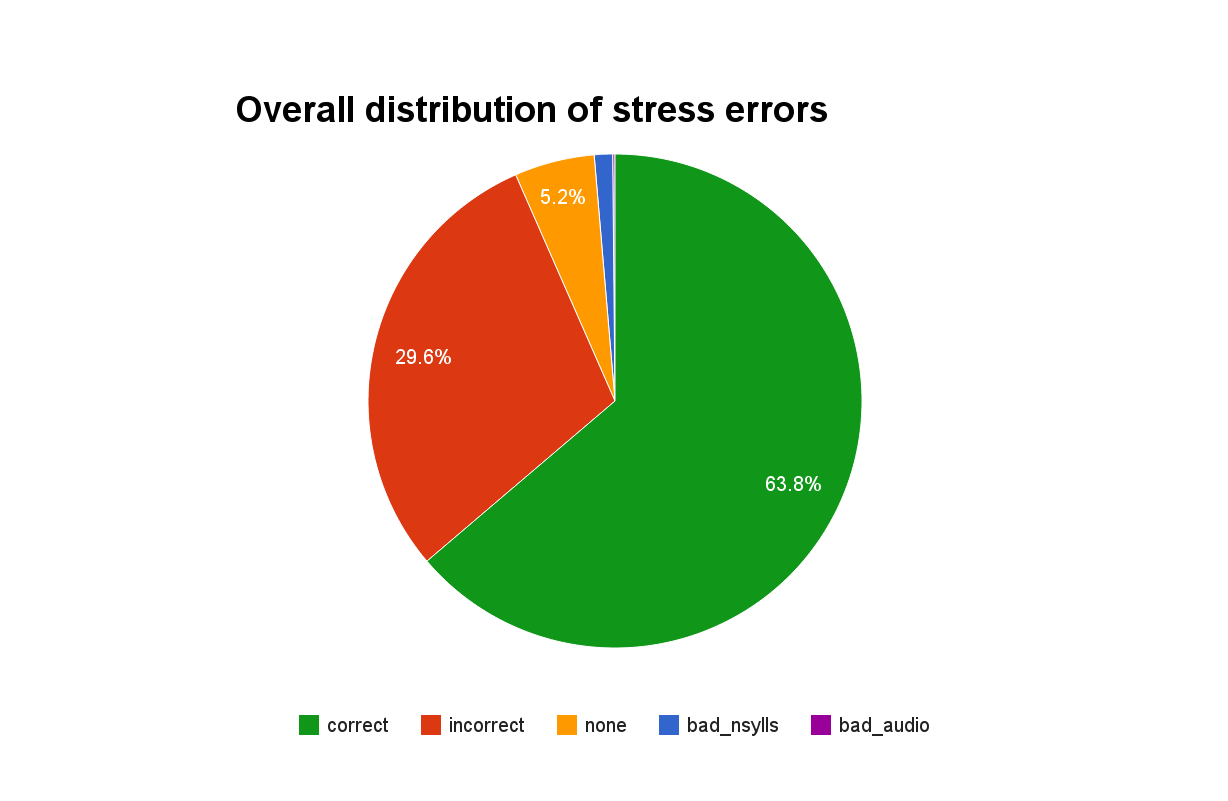
\includegraphics[width=\textwidth]{img/annotation/overallPie}
%			\caption{Overall distribution of lexical stress errors in the annotated corpus \TODO{retitle}}
%			\label{fig:results:overallpie}
%		\end{figure}
		
		\begin{figure}[ht]
			\centering
			\caption{Overall distribution of lexical stress errors in the annotated data}
			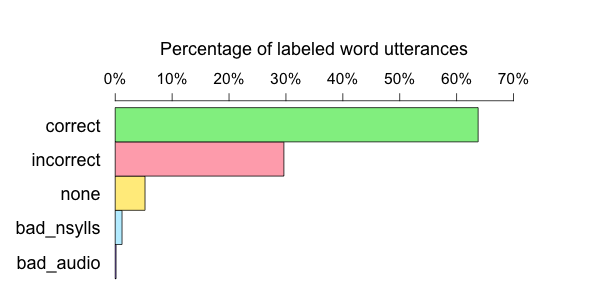
\includegraphics[width=.7\textwidth]{img/plots/overallJudgments-axisTop-noLabels}
			\label{fig:results:overallbars}
		\end{figure}
		
		
		
		This sizable proportion of errors seems to give an affirmative answer to the question of whether lexical stress errors are observed frequently in L2 German speech by L1 French speakers. Bearing in mind that frequency of production is one of the criteria mentioned in \cref{sec:targeting:frequency} above for choosing a good error to target with CAPT, this provides further justification of the choice of lexical stress errors as the error type to focus on in this thesis project.
		
		%\subsubsection{Accuracy by word type}
		\subsection{Errors by word type}
		\label{sec:results:wordtype}
			
			To take a more detailed look at the errors observed in the annotated data, error judgments were broken down by word type, with the results of this analysis presented in \cref{tab:results:wordtype} and illustrated in \cref{fig:results:wordbars}. 
			
			
			
%			\begin{table}[tbp]
%				\centering
%				\caption[Errors by word type]{Errors by word type \TODO{put \%s in parens and lose 2nd row} \TODO{omit 0 values?}}
%				\begin{tabularx}{\textwidth}{lrXrXrXrXrX}
%				\toprule
%				Word type & \multicolumn{2}{c}{correct}		& \multicolumn{2}{c}{incorrect} &		\multicolumn{2}{c}{none} &		\multicolumn{2}{c}{bad\_nsylls} & 		\multicolumn{2}{c}{bad\_audio} \\	
%				& $N$ & \% & $N$ & \% & $N$ & \% & $N$ & \% & $N$ & \% \\
%					\midrule
%E-mail &	35	& 62.50\%	&21&	37.50\%&	0	&0.00\%&	0	&0.00\%	& 0	& 0.00\% \\
%Flagge	& 33	&60.00\%	 &	16	 &	29.09\%	 &	6	 &	10.91\%	 &	0	 &	0.00\%	 &	0	 &	0.00\%\\
%fliegen &	46	&82.14\%	 &	7	 &	12.50\% &		1	 &	1.79\% &		2	 &	3.57\%	 &	0	 &	0.00\%\\
%Fr\"{u}hling &	48&	85.71\% &		7	 &	12.50\% &		1 &		1.79\%	 &	0	 &	0.00\% &		0	 &	0.00\%\\
%halten &	35	&62.50\%	 &	19	 &	33.93\%	 &	2 &		3.57\%	 &	0	 &	0.00\%	 &	0	 &	0.00\%\\
%manche&	36	&64.29\%	 &	17	 &	30.36\%	 &	1	 &	1.79\%	 &	1	 &	1.79\% &		1	 &	1.79\%\\
%M\"{o}rder	&33&	58.93\%	 &	16	 &	28.57\%	 &	7	 &	12.50\%	 &	0	 &	0.00\%	 &	0	 &	0.00\%\\
%Pollen	& 36	&64.29\%	 &	19	 &	33.93\%	 &	1	 &	1.79\%	 &	0	 &	0.00\%	 &	0	 &	0.00\%\\
%Ringen	& 32	&58.18\%	 &	12	 &	21.82\%	 &	8	 &	14.55\%	 &	3	 &	5.45\%	 &	0	 &	0.00\%\\
%Tatort	& 20	&36.36\%	 &	32	 &	58.18\%	 &	2	 &	3.64\%	 &	1	 &	1.82\%	 &	0	 &	0.00\%\\
%tragen	& 32	&58.18\%	 &	23	 &	41.82\%	 &	0	 &	0.00\%	 &	0	 &	0.00\%	 &	0	 &	0.00\%\\
%Tschechen &	40	&71.43\%&	9	 &	16.07\%	 &	6	 &	10.71\%	 &	1	 &	1.79\% &		0	 &	0.00\% \\
%					\bottomrule
%				\end{tabularx}
%				\label{fig:results:wordtype}
%			\end{table}
			
			\begin{table}[tbp]
				\centering
				\caption[Errors by word type]{Errors by word type: Number of tokens (utterances) assigned to each of the five categories, listed by word type. Equivalent percentages of each word type's total number of tokens are given in parentheses.}
				\begin{tabularx}{\textwidth}{lXXXXX}
				\toprule
				Word & correct & incorrect & none & bad\_nsylls & bad\_audio \\	
					\midrule
E-mail 			&	35 (62.5\%)	& 21 (37.5\%) 	&	0 					&	0 				&  0  				\\
Flagge			& 33 (60.0\%)	&	16 (29.1\%)	&	6 (10.9\%)	&	0 		 		&	0 					\\
fliegen 			&	46 (82.1\%)	&	7 (12.5\%) 	&	1 (1.8\%) 		&	2 (3.6\%)	&	0 					\\
Fr\"{u}hling 	&	48 (85.7\%) 	&	7 (12.5\%) 	&	1 (1.8\%)		&	0 				&	0 					\\
halten 			&	35 (62.5\%)	&	19 (33.9\%)	&	2 (3.6\%)		&	0				&	0 					\\
manche		&	36 (64.3\%)	&	17 (30.4\%)	&	1 (1.8\%)		&	1 (1.8\%) 	&	1 (1.79\%)	\\
M\"{o}rder	& 33 (58.9\%)	&	16 (28.6\%)	&	7 (12.5\%)	&	0 				&	0 					\\
Pollen			& 36 (64.3\%)	&	19 (33.9\%)	&	1 (1.8\%)		&	0 				&	0 					\\
Ringen			& 32 (58.2\%)	&	12 (21.8\%)	&	8 (14.6\%)	&	3 (5.5\%)	&	0 					\\
Tatort			& 20 (36.4\%)	&	32 (58.2\%)	&	2 (3.6\%)		&	1 (1.8\%)	&	0 					\\
tragen			& 32 (58.2\%)	&	23 (41.8\%)	&	0 					&	0 				&	0 					\\
Tschechen 	&	40 (71.4\%)	&	9 (16.1\%)	 &	6 (10.7\%)	&	1 (1.8\%) 	&	0  				\\
					\bottomrule
				\end{tabularx}
				\label{tab:results:wordtype}
			\end{table}
			
%			\begin{figure}[htb]
%				\centering
%				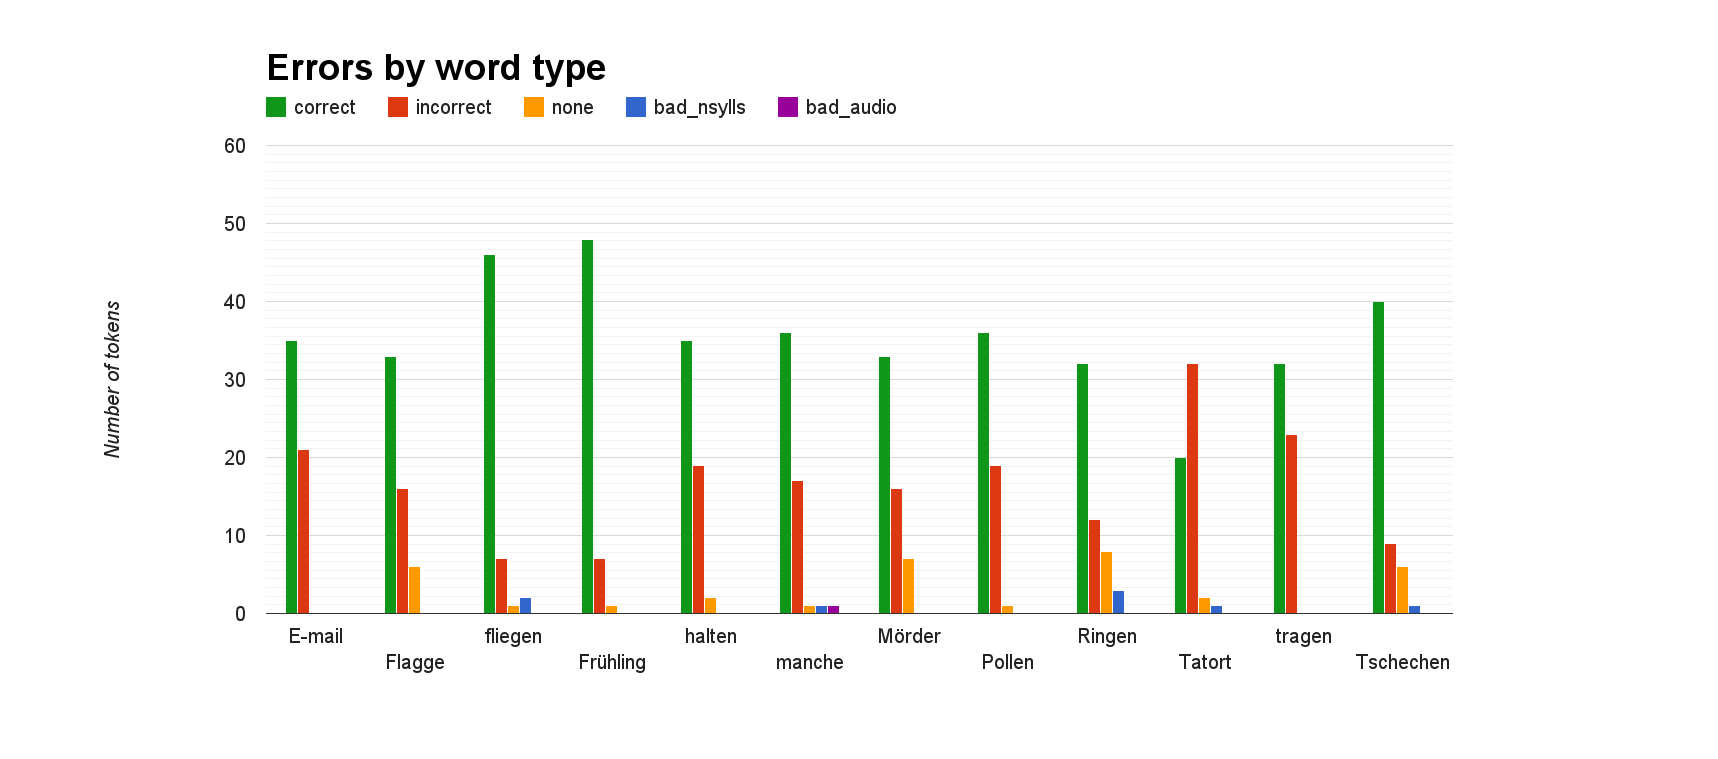
\includegraphics[width=\textwidth]{img/annotation/wordBars}
%				\caption{Errors by word type}
%				\label{fig:results:wordbars}
%			\end{figure}		

			\begin{figure}[htbp]
				\centering
				\caption[Error distribution by word type]{Distribution of errors by word type,
				as a percentage of the total number of labeled tokens (utterances) of that word type 
				(see \cref{tab:results:wordtypes} for precise values)
				}
				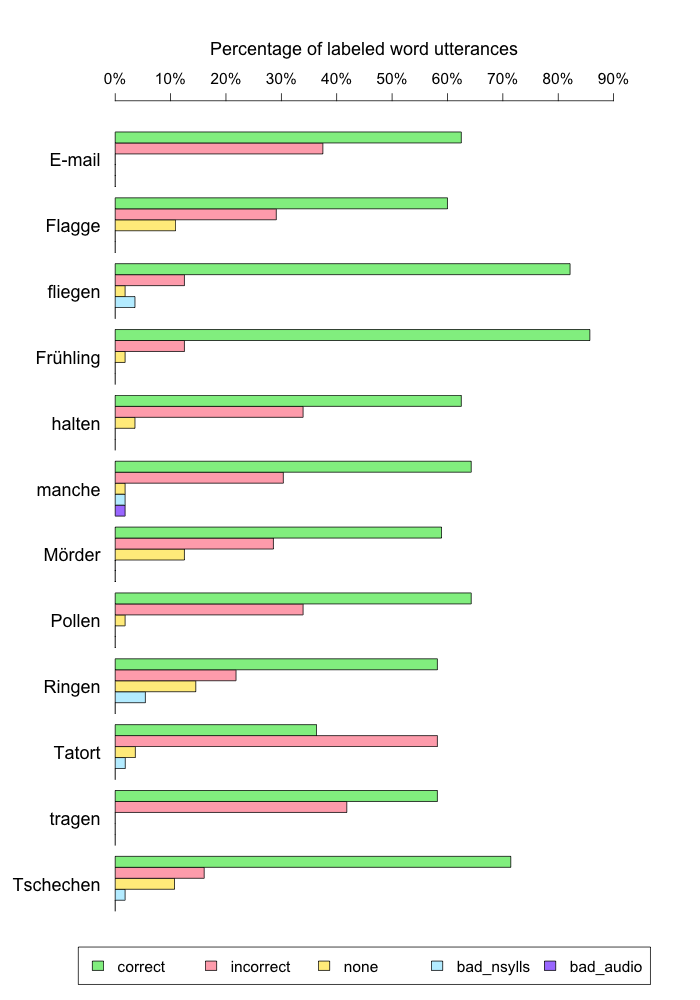
\includegraphics[width=\textwidth]{img/plots/judgmentsWordTypes}
				\label{fig:results:wordbars}
			\end{figure}	
			
			As should be expected, most word types exhibit a distribution of errors quite similar to the overall distribution, i.e. a ratio of correct to incorrect utterances of approximately 2:1, broadly speaking. However, for the words \textit{fliegen}, \textit{Fr\"{u}hling}, and \textit{Tschechen}, a much higher proportion of correct stress realizations was observed,
			%For the word \textit{tragen}, the number of incorrect realizations (23, or 41.82\%)was much closer to that of correct ones  (32, or 58.18\%) , 
			and for one word, \textit{Tatort}, incorrect realizations actually exceeded correct productions by a noticeable margin (32 or 58.18\% versus 20 or 36.36\%, respectively). 
			
			Unfortunately, no clear explanations for these discrepancies between word types readily present themselves, though a few speculations will be offered here. Of the words with uncommonly high proportions of correct utterances, two of the three (\textit{fliegen} and \textit{Fr\"{u}hling}) occurred in the same sentence in the IFCASL corpus --  \textit{In Fr\"uhling fliegen Pollen durch die Luft} -- along with another of the annotated word types, \textit{Pollen}. This sentence, in part due to the occurrence of these three bisyllabic initial-stress words in immediate succession, exhibits a very regular metrical pattern:
			%TODO {is this iambic or trochaic? explanation? reference?}:
			\begin{center}
			\begin{tabular}{llllllllll}
			In & Fr\"uh-& ling & flie-& gen & Pol-& len & durch & die & Luft \\
			- & x & - &  x & - & x & - & x & - & x \\
			\end{tabular}
			\end{center}
			As a result of this regularity, correctly realizing the prosody of each word in this sentence may present less of a challenge to L1 French speakers than a less regular sentence, and may thus explain their uncharacteristically flawless productions of the words therein. The fact that no fewer than the expected proportion of errors were observed in utterance of \textit{Pollen} would seem to contradict this speculative explanation; however, unlike the other words, \textit{Pollen} is doubly challenging for L1 French speakers, insofar as its first vowel is a short \textipa{O}, as opposed to the long \textipa{o:} in the word \textit{Polen} (meaning \textit{Poland} in English), with which \textit{Pollen} forms a minimal pair.\footnote{This minimal pair was of interest to the researchers who constructed the IFCASL corpus, and \textit{Polen} also appears in the corpus, though it was not selected for inclusion in the sub-corpus to be annotated for lexical stress errors.}  Differentiating between long and short vowels when speaking German is a notorious hurdle for French speakers \TODO{reference(s)}. It may be the case that the short vowel in \textit{Pollen}, and the existence of another similar-sounding word, is responsible for some of the errors observed in the data, even though \textit{Pollen} and \textit{Polen} share the same stress pattern (stress on the initial syllable), for one of two reasons: either the added challenge of producing a difficult vowel in \textit{Pollen} distracts French speakers from the simple, regular prosody of the sentence, causing them to produce more prosodic errors with this word, or the native German annotators (most of whom, as discussed in \cref{sec:lexstress:annotators}, are not trained in phonetics or phonology) who are tasked with assessing the correctness of the word's prosody are distracted by the incorrect vowel quantity/quality in French speakers' productions of this word, and erroneously interpret the flaw(s) that they detect in the word's pronunciation as having to do with lexical stress, when in fact they are segmental errors. 
			\TODO{...or it could be word frequency (Pollen less frequent), or maybe influence of phrase position or interpreted phrase position, cf. \citep{Michaux2013}?}
			
			As for the uncharacteristically large proportion of errors in \textit{Tatort}, it may be the case that this word's resemblance to the common French words \textit{ta} (\textit{your}) and \textit{tort} (\textit{wrong}) interferes with French speakers' production, such that they realize the word as the plausible French word sequence \textit{ta tort} (\textit{your wrong(doing)} or \textit{your mistake}), in which \textit{tort} would unmistakably be the focus \TODO{is that inaccurate?}, instead of realizing it correctly as a compound of the German words \textit{Tat} (\textit{act}) and \textit{Ort} (\textit{place}).
			%, its actual meaning in German being \textit{crime scene}.
			However, once again it should be noted that this
			% explanation is purely speculative
			%and 
			purely speculative explanation is not (and cannot be) verified by the data collected here.  
			
			\TODO{outro?}
			
			
		
		
		
		%\subsubsection{Accuracy by L2 skill level}
		\subsection{Errors by L2 proficiency level}
		\label{sec:results:level}
		
		
		
			\TODO{Be consistent with skill/proficiency or OK to use them interchangeably?}
			
			As \cref{sec:lexstress:data} stated, the L1 French speakers whose recordings comprise the annotated IFCASL sub-corpus span four levels of L2 German proficiency: A2 (elementary), B1 (intermediate), B2 (upper intermediate), and C1 (advanced). The rightmost column of \cref{tab:results:levels} gives the number and proportion of utterances from speakers of each level in the annotated sub-corpus, along with the number of utterances from speakers of each level that were assigned to each of the five possible stress-accuracy labels, and these figures are illustrated in \cref{fig:levelbars:4}. Because the total number of utterances by speakers of each of the two intermediate (B) levels in the corpus is lower than the number by speakers of the lowest (A2) and highest (C1) levels, the judgments have also been grouped into two broader categories for easier comparison: beginners (A2 and B1) and advanced speakers (B2 and C1). The breakdown of stress errors by these groups is given in the lower portion of \cref{tab:results:levels} and illustrated in \cref{fig:levelbars:groups}.
			
			
			
%			\begin{table}
%				\begin{tabularx}{\textwidth}{XrXrXrXrXrXr}		
%				\toprule
%				 & \multicolumn{2}{c}{correct}		& \multicolumn{2}{c}{incorrect} &		\multicolumn{2}{c}{none} &		\multicolumn{2}{c}{bad\_nsylls} & 		\multicolumn{2}{c}{bad\_audio} & Total (\%) \\
%				\midrule			
%A2	&	137	&	47.74\%	&	118	&	41.11\%	&	26	&	9.06\%	&	5	&	1.74\%	&	1	&	0.35\%	&	287	(42.96\%)	\\
%B1	&	68	&	56.67\%	&	49	&	40.83\%	&	3	&	2.50\%	&	0	&	0.00\%	&	0	&	0.00\%	&	120 (17.96\%)	\\
%B2	&	52	&	72.22\%	&	17	&	23.61\%	&	3	&	4.17\%	&	0	&	0.00\%	&	0	&	0.00\%	&	72	(10.78\%)	\\
%C1	&	169	&	89.42\%	&	14	&	7.41\%	&	3	&	1.59\%	&	3	&	1.59\%	&	0	&	0.00\%	&	189	(28.29\%)	\\
%				\bottomrule
%				\end{tabularx}
%			\end{table}		

%		\begin{table}
%			\caption{Errors by speaker skill level}
%				\begin{tabularx}{\textwidth}{XXXXXXX}		
%				\toprule
%				 & correct	& incorrect &	none &		bad\_nsylls & 		{bad\_audio} & %\multicolumn{2}{c}{Total (\% corpus)} 
%				 \\
%				\midrule			
%A2	&	137	(47.7\%)	&	118	(41.1\%)	&	26 (9.1\%)	&	5	(1.7\%)		&	1	(0.4\%)		&	287	(43.0\%)	\\
%B1		&	68	(56.7\%)	&	49 	(40.8\%)	&	3	(2.5\%)		&	0					&	0					&	120	(18.0\%)	\\
%B2		&	52	(72.2\%) &	17	(23.6\%)	&	3	(4.2\%)		&	0					&	0					&	72	(10.8\%)	\\
%C1	&	169	(89.4\%) &	14	(7.4\%)		&	3	(1.6\%)		&	3	(1.6\%)		&	0					&	189	(28.3\%)	\\
%				\midrule					
%Beginner (A2,B1)	&	205	(50.4\%)	&	167	(41.0\%)	&	29 (7.1\%)	&	5	(1.2\%)	&	1	(0.3\%)	&	407	(60.9\%)	\\
%Advanced (B2,C1)	&	221	(84.7\%)	&	31	(11.9\%)	&	6	(2.3\%)	&	3	(1.2\%)	&	0					&	261	(39.1\%)	\\
%				\bottomrule
%				\end{tabularx}
%				\label{tab:results:levels}
%			\end{table}		
			
		\begin{table}
			\caption[Errors by L2 proficiency level]{Errors by L2 proficiency level: Number of tokens (utterances) assigned to each of the five categories, listed by the L2 German proficiency level of the speaker. Equivalent percentages of the total number of tokens for each level/level group are given in parentheses.}
			\setlength{\tabcolsep}{0.5mm}
			
			\begin{subtable}{\textwidth}
				\caption{Individual levels}
				\begin{tabularx}{\textwidth}{lrXrXrXrX}
				\toprule
					&	A2 & %\multicolumn{2}{l}{A2}					
					&	B1 & %\multicolumn{2}{l}{B1}						
					&	B2 & %\multicolumn{2}{l}{B2}							
					&	C1 & %\multicolumn{2}{l}{C1}					
					\\
				\midrule
correct			&	137 	& (47.7\%)	&	68	& (56.7\%)	&	52	& (72.2\%)	&	169	& (89.4\%)	\\
incorrect		&	118 	& (41.1\%)	&	49	& (40.8\%)	&	17	& (23.6\%)	&	14	& (7.4\%)		\\
none				&	26 	& (9.1\%)		&	3		& (2.5\%)		&	3		& (4.2\%)		&	3		& (1.6\%)		\\
bad\_nyslls	&	5		& (1.7\%)		&	0		&					&	0		&					&	3		& (1.6\%)		\\
bad\_audio	&	1		& (0.4\%)		&	0		&					&	0		&					&	0		&					\\
Total (\% of dataset)	&	287 & (43.0\%)	&	120 & (18.0\%)	&	72 & (10.8\%)	&	189 & (28.3\%)	\\
				\bottomrule
				\end{tabularx}
				\label{tab:results:levels:4}
			\end{subtable}
			
			\vspace{1em}
			
			\begin{subtable}{\textwidth}
				\caption{Level groups}
				\begin{tabularx}{\textwidth}{XrXrX}
				\toprule
					&	\multicolumn{2}{l}{Beginner (A2+B1)}					
					&	\multicolumn{2}{l}{Advanced (B2+C1)}									
					\\
				\midrule
correct			&	205	&	(50.37\%)	& 221	&	(84.67\%)	\\
incorrect		&	167	&	(41.03\%) & 31		&	(11.88\%)\\
none				&	29	&	(7.13\%)	& 6		&	(2.30\%)\\
bad\_nyslls	&	5		&	(1.23\%)	& 3		&	(1.15\%)\\
bad\_audio	&	1		&	(0.25\%) 	& 0		& 	\\
Total (\% of dataset)	&	407	&	(60.93\%) & 261	&	(39.07\%)	\\
				\bottomrule
				\end{tabularx}
				\label{tab:results:levels:groups}
			\end{subtable}
			
			\label{tab:results:levels}
		\end{table}
					
			
			\begin{figure}[tbp]
				\centering
				%\caption{Stress judgments by speaker skill level}
				\caption[Error distribution by proficiency level]{Distribution of errors by speaker's L2 German proficiency level,
				as a percentage of the total number of labeled tokens (utterances) from speakers of that level/group 
				(see \cref{tab:results:levels} for precise values)
				}
				\begin{subfigure}{\textwidth}
					\centering
					\caption{Each level}
					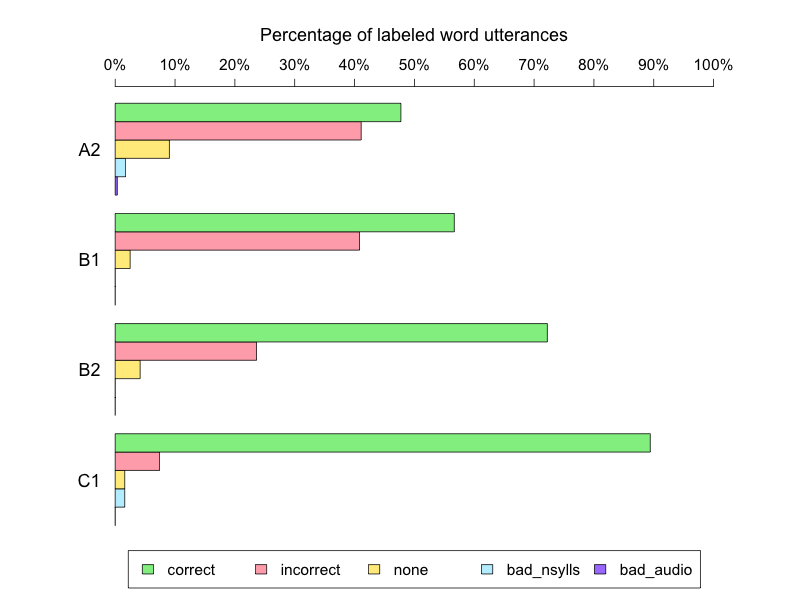
\includegraphics[width=\textwidth]{img/plots/judgments4Levels}
					\label{fig:levelbars:4}
				\end{subfigure}

				\vspace{1em}				
				
				\begin{subfigure}{\textwidth}
					\centering
					\caption{Level groups (Beginner is A2 + B1, Advanced is B2 + C1)}
					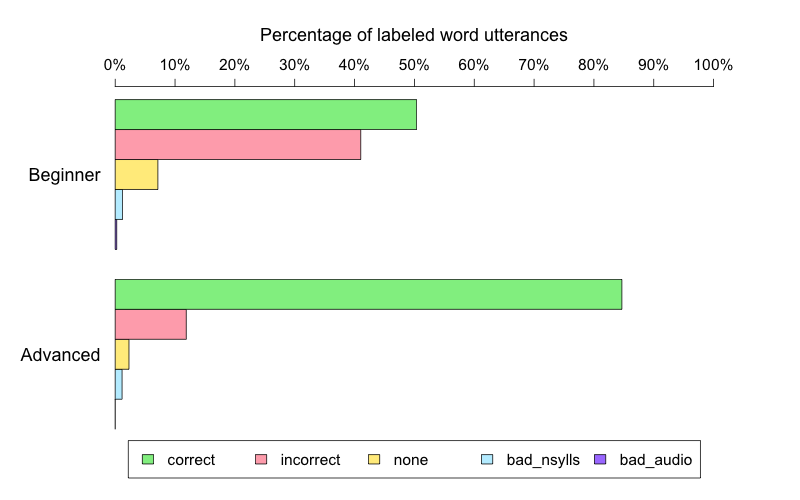
\includegraphics[width=\textwidth]{img/plots/judgmentsLevelGroups}
					\label{fig:levelbars:groups}
				\end{subfigure}
				
				\label{fig:levelbars}
			\end{figure}
			
%			
%			\begin{figure}[ht]
%				\centering
%				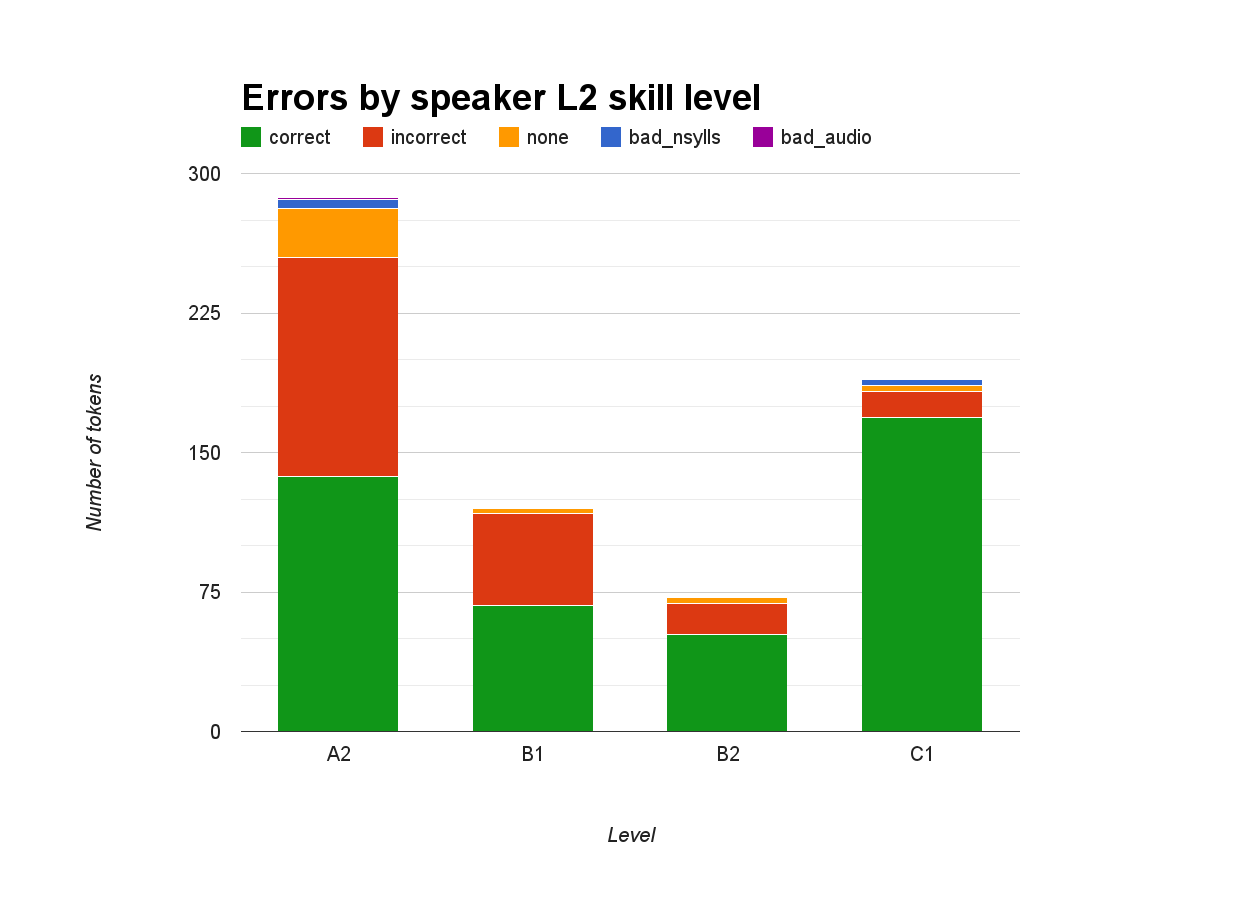
\includegraphics[width=\textwidth]{img/annotation/skillLevelBars}
%				\caption{Stress judgments by speaker skill level \TODO{Exclude?}}
%				\label{fig:levelbars}
%			\end{figure}
		
		
%			\begin{figure}[htb]
%				\centering
%				\begin{subfigure}[t]{0.5\textwidth}
%					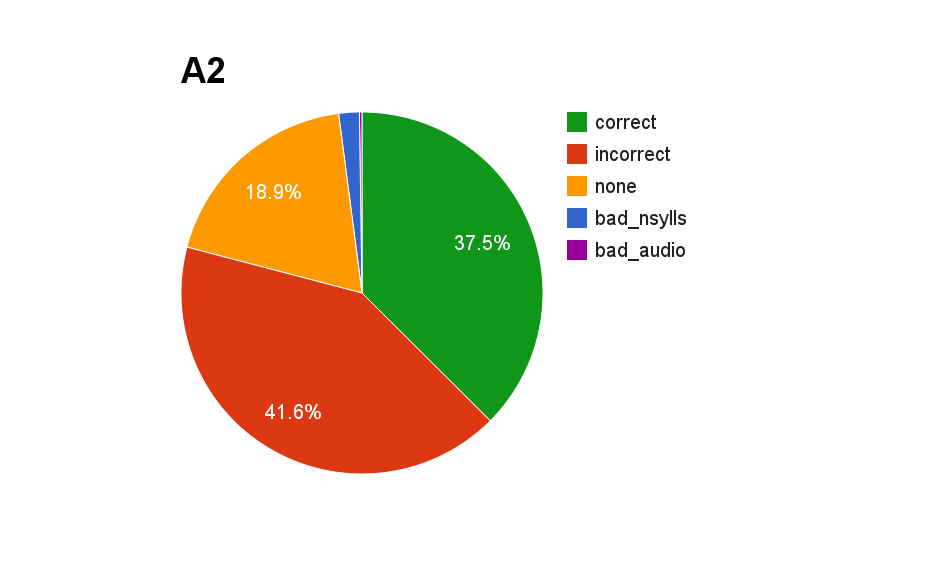
\includegraphics[width=\textwidth]{img/annotation/A2}
%					\caption{A2}
%					\label{fig:levelpies:A2}
%				\end{subfigure}%
%				~
%				\begin{subfigure}[t]{0.5\textwidth}
%					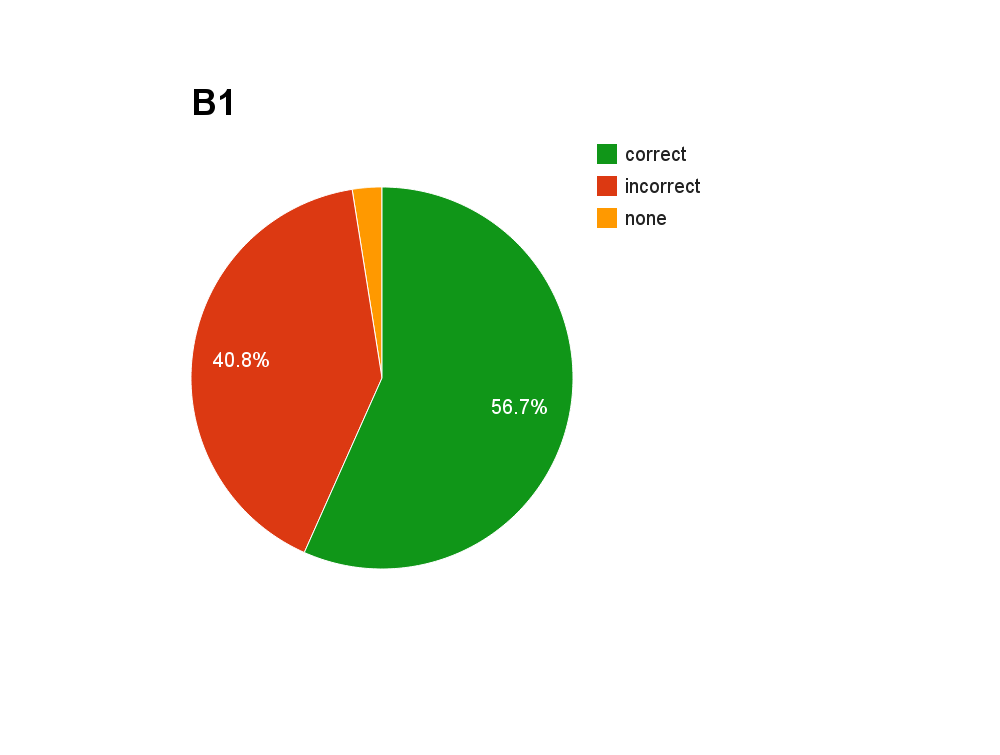
\includegraphics[width=\textwidth]{img/annotation/B1}
%					\caption{B1}
%					\label{fig:levelpies:B1}
%				\end{subfigure}%
%				
%				\begin{subfigure}[b]{0.5\textwidth}
%					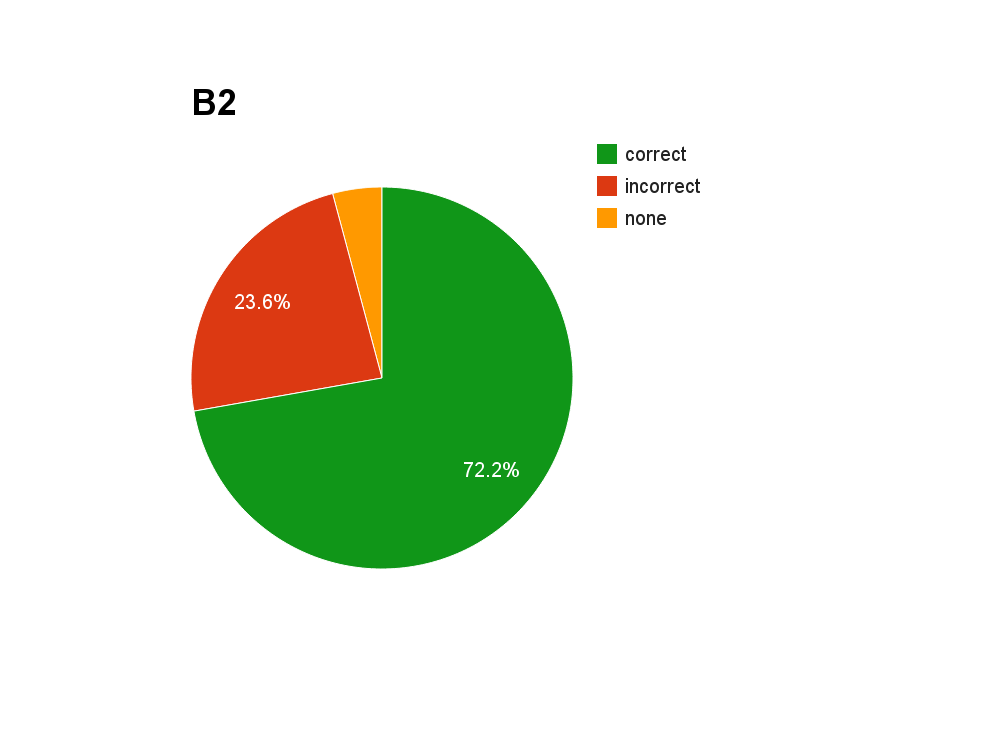
\includegraphics[width=\textwidth]{img/annotation/B2}
%					\caption{B2}
%					\label{fig:levelpies:B2}
%				\end{subfigure}%
%				~
%				\begin{subfigure}[b]{0.5\textwidth}
%					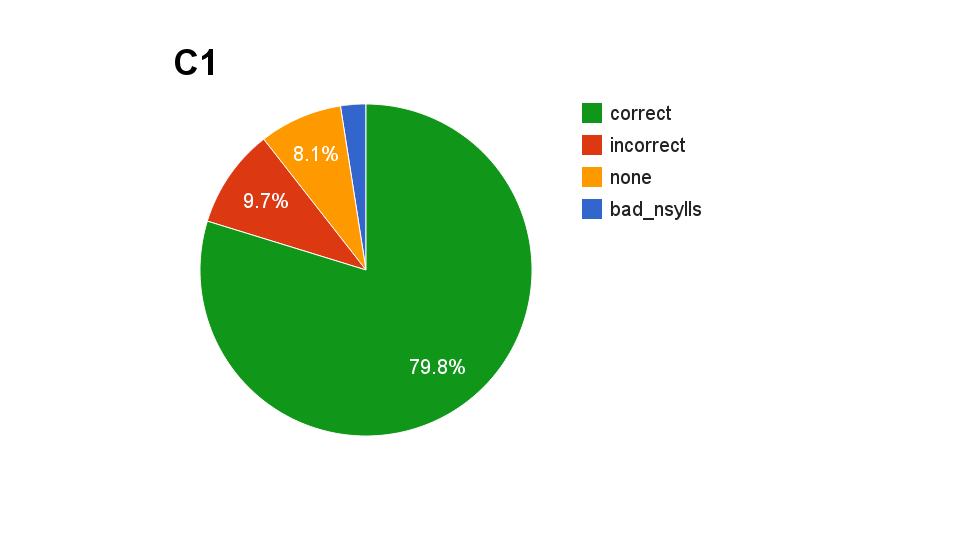
\includegraphics[width=\textwidth]{img/annotation/C1}
%					\caption{C1}
%					\label{fig:levelpies:C1}
%				\end{subfigure}%
%				\caption{Error distribution by speaker skill level}
%				\label{fig:levelpies}
%			\end{figure}		
			
			
			
			
			
			
%			\begin{table}
%			\begin{tabularx}{\textwidth}{lrXrXrXrXrXrX}		
%			\toprule
%			Group & \multicolumn{2}{c}{correct}		& \multicolumn{2}{c}{incorrect} &		\multicolumn{2}{c}{none} &		\multicolumn{2}{c}{bad\_nsylls} & 		\multicolumn{2}{c}{bad\_audio} & Total & \% of corpus \\
%			\midrule			
%				
%			\bottomrule
%			\end{tabularx}
%			\end{table}		
			
%			\begin{figure}[htb]
%				\centering
%				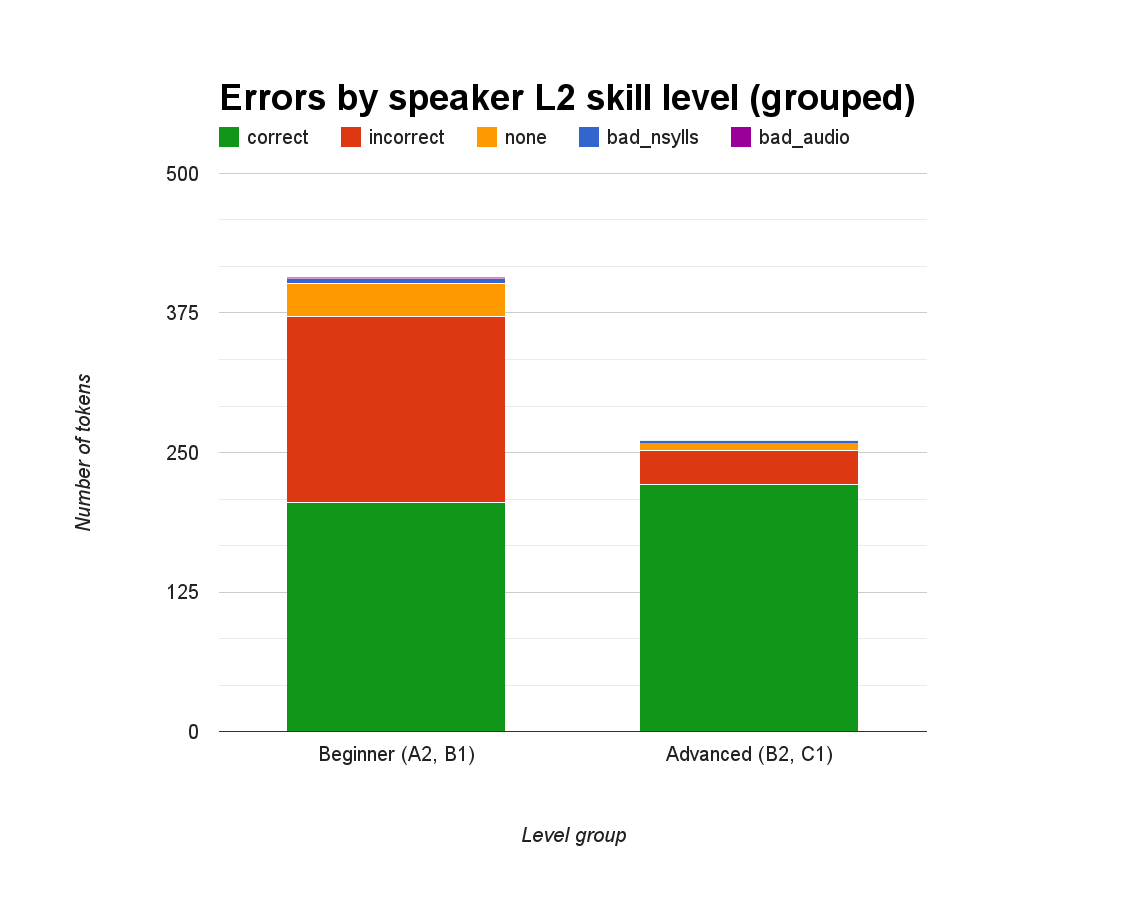
\includegraphics[width=\textwidth]{img/annotation/skillLevelGroupsBars}
%				\caption{Stress judgments by speaker skill level (grouped)}
%				\label{fig:levelgroupsbars}
%			\end{figure}
%			
%			
%			\begin{figure}[htb]
%				\centering
%				\begin{subfigure}[t]{0.5\textwidth}
%					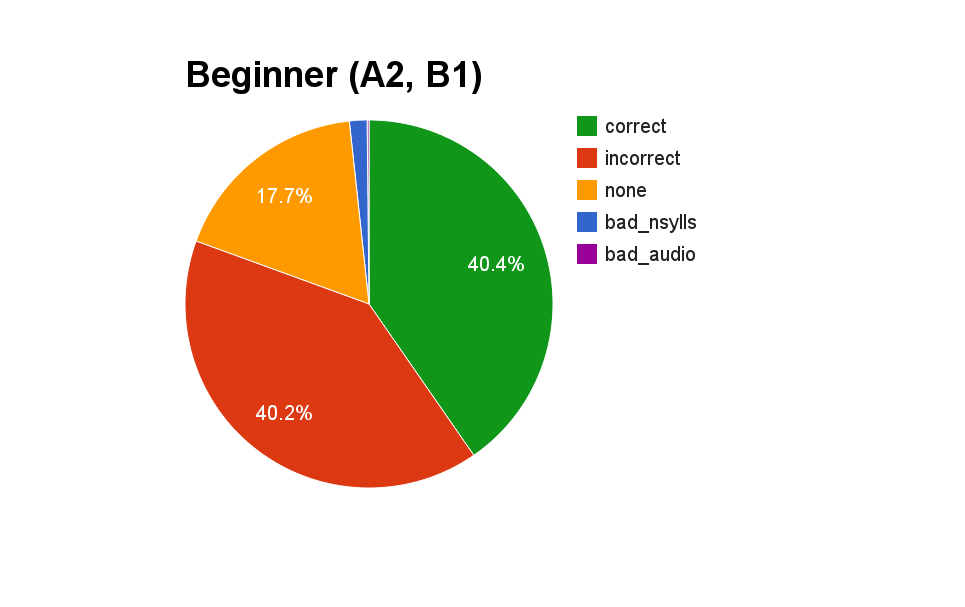
\includegraphics[width=\textwidth]{img/annotation/beginnerPie}
%					\caption{}
%					\label{fig:levelgroupspies:beg}
%				\end{subfigure}%
%				~
%				\begin{subfigure}[t]{0.5\textwidth}
%					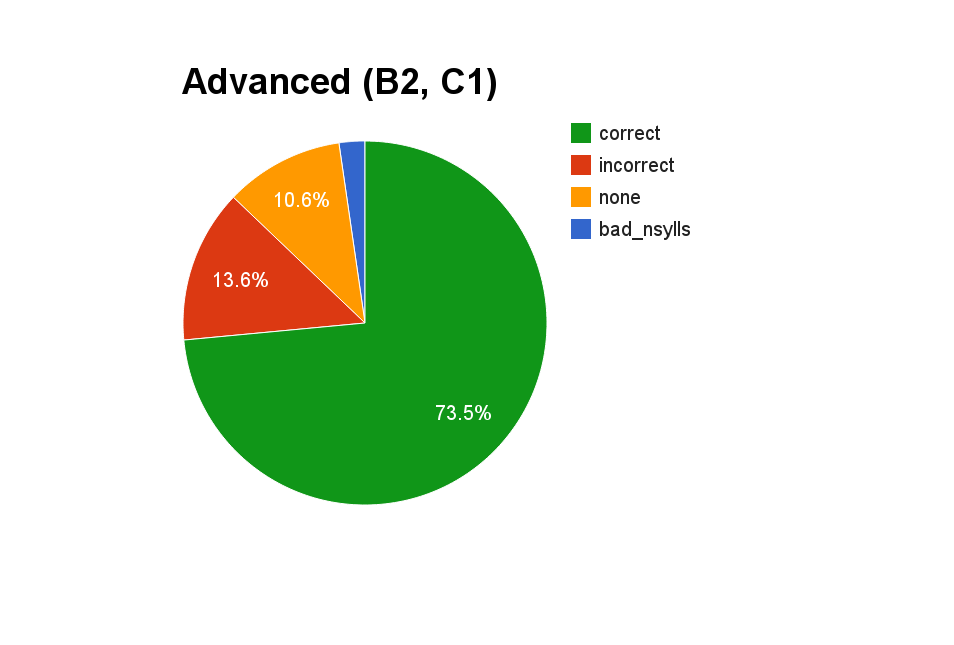
\includegraphics[width=\textwidth]{img/annotation/advancedPie}
%					\caption{}
%					\label{fig:levelgroupspies:adv}
%				\end{subfigure}%
%				\caption{Error distribution by speaker skill level (grouped)}
%				\label{fig:levelgroupspies}
%			\end{figure}	
			
			
	Unsurprisingly, these figures reveal that  speakers of the higher levels (B2 and C1) seem to make a proportionally lower number of errors than speakers of the lower ones (A2 and B1), with each level exhibiting a lower proportion of errors than the level below it. Generally speaking, beginners  (A2 and B1) seem to realize lexical stress correctly in about half of their utterances, whereas for upper intermediate (B2) learners the proportion of correct utterances is closer to three-fourths, and it approaches 90\% for advanced (C1) learners. As previously established (see \cref{sec:bkgd:targeting}), a CAPT system targeting a particular type of error will only be useful if that error is produced with considerable frequency by the learners using the system; therefore, it would seem from the frequency of lexical stress errors in their speech that learners of lower proficiency levels may benefit more from a CAPT system targeting such errors than learners of higher proficiency. 
			\TODO{This conforms with findings of \textcite{Michaux2012} that beginners make more errors than advanced learners.}
			
			
		
		\subsection{Errors by speaker age and gender}
		\label{sec:results:agegender}
			
			
			Given that the IFCASL corpus, and by extension the sub-corpus annotated for lexical stress errors, contains recordings from speakers of both genders and from adult speakers (those over age 18 \TODO{check that}) as well as children (see \cref{sec:lexstress:data}), an analysis of the errors observed in terms of the age and gender of the speakers is of interest, to determine whether any discernible differences exist between the different groups of speakers. The breakdown of errors for each of these groups is presented in \cref{tab:results:agegender} and illustrated in \TODO{\cref{fig:results:agepies,fig:results:genderpies}}.
			
			
			\begin{table}[p]
			\caption[Errors by speaker age and gender]{Errors by speaker age and gender: Number of tokens (utterances) assigned to each of the five categories, listed by the age/gender of the speaker. Equivalent percentages of the total number of tokens for each age/gender group are given in parentheses.}
			\setlength{\tabcolsep}{0.5mm}
			
			\vspace{1em}			
			
			\begin{subtable}{\textwidth}
				\centering
				\caption{Individual age/gender categories. Boys and Girls are males and females under the age of 18, respectively, and Men and Women are males and females over 18, respectively.}
				\begin{tabularx}{\textwidth}{lrXrXrXrX}
				\toprule
				& \multicolumn{2}{c}{Boys}% &
				& \multicolumn{2}{c}{Girls}% &
				& \multicolumn{2}{c}{Men}% &
				& \multicolumn{2}{c}{Women}% &
				\\
				\midrule
correct			&	48	&	(36.64\%)	&	6		&	(25.00\%)	&	184	&	(73.02\%)	&	188	&	(72.03\%)	\\
incorrect		&	60	&	(45.80\%)	&	17	&	(70.83\%)	&	61	&	(24.21\%)	&	60	&	(22.99\%)	\\
none				&	17	&	(12.98\%)	&	1		&	(4.17\%)	&	7		&	(2.78\%)	&	10	&	(3.83\%)	\\
bad\_nsylls	&	5		&	(3.82\%)	&	0		&					&	0		&					&	3		&	(1.15\%)	\\
bad\_audio	&	1		&	(0.76\%)	&	0		&					&	0		&					&	0		&		\\
Total (\%) of corpus)	&	131	&	(19.61\%)	&	24	&	(3.59\%)	&	252	&	(37.72\%)	&	261	&	(39.07\%)	\\
				\bottomrule
				\end{tabularx}
			\end{subtable}			
			
			\vspace{2em}
			
			\begin{subtable}{\textwidth}
				\centering
				\caption{By age, regardless of gender. Children are adolescents under age 18, adults are over 18. Adult beginners are adults with a German proficiency level of A2 or B1.}
				\begin{tabularx}{\textwidth}{lrXrXrX}
				\toprule
				& \multicolumn{2}{l}{Children}
				& \multicolumn{2}{l}{Adults}
				& \multicolumn{2}{l}{Adult beginners}
				\\
				\midrule
correct			&	54	&	(34.84\%)	&	372	&	(72.51\%)	&	151	&	(59.92\%)	\\
incorrect		&	77	&	(49.68\%)	&	121	&	(23.59\%)	&	90	&	(35.71\%)	\\
none				&	18	&	(11.61\%)	&	17	&	(3.31\%)	&	11	&	(4.37\%)	\\
bad\_nsylls	&	5		&	(3.23\%)	&	3		&	(0.58\%)	&	0		&		\\
bad\_audio	&	1		&	(0.65\%)	&	0		&					&	0		&		\\
Total (\%) of corpus)	&	155	&	(23.20\%)	&	513	&	(76.80\%)	&	252	&	(37.72\%)	\\
				\bottomrule
				\end{tabularx}
			\end{subtable}
			
			\vspace{2em}
			
			\begin{subtable}{\textwidth}
				%\centering
				\caption{By gender, regardless of age.}
				\begin{tabularx}{\textwidth}{XrXrX}
				\toprule
					&	\multicolumn{2}{l}{Males}					
					&	\multicolumn{2}{l}{Females}									
					\\
				\midrule
correct			&	232	&	(60.57\%)	&	194	&	(68.07\%)	\\
incorrect		&	121	&	(31.59\%)	&	77	&	(27.02\%)	\\
none				&	24	&	(6.27\%)	&	11	&	(3.86\%)	\\
bad\_nsylls	&	5		&	(1.31\%)	&	3		&	(1.05\%)	\\
bad\_audio	&	1		&	(0.26\%)	&	0		&		\\
Total (\% of corpus)	&	383	&	(57.34\%)	&	285	&	(42.66\%)	\\
				\bottomrule
				\end{tabularx}
			\end{subtable}
			
			\label{tab:results:agegender}
			\end{table}
			
			

				With regard to the two different age groups of speakers, any interpretation of the results presented here must bear in mind the considerable difference in size between the two different groups: \TODO{reference the actual number of each type of speaker - should already have been presented in \cref{sec:lexstress:data} or earlier} of the 668 tokens annotated in total, 513 (over three-fourths) were from adult speakers while only 155 (less than one-fourth) were utterances by children. Furthermore, it must be highlighted that there is a strong interaction between age and proficiency level: all of the child speakers recorded in the IFCASL corpus are beginners 
				(the majority at the A2 level with only 1 girl at B1),
				% \TODO{technically true but implies A2 while a couple of the girls are B1 - worth mentioning?}, 
				while the adults span all four levels. Given the discrepancies between L2 proficiency levels discussed in the previous section, then, it is not surprising to see that over half of children's utterances are judged to have lexical stress errors, with correct stress productions making up only 35.1\% of utterances (54 utterances) by this age group. Adults, on the other hand, seem to realize lexical stress correctly in the majority of their utterances, with only 23.6\% (121) incorrect productions and 3.3\% percent (17) utterances with no clear lexical stress realization ([none]). However, this is not an entirely just comparison, given that the group of child speakers only includes beginners; therefore, instead of comparing the children's error distribution to that of all adults, it is helpful to restrict the comparison to adults of the lower proficiency levels. 
				%The bottom rows of \cref{tab:results:agegender} list
				\Cref{tab:results:agegender} lists the statistics for 
				\TODO{\textit{remove?:} adults at the A2 proficiency level only as well as for}
				adults of both beginner levels (A2 and B1), 
				and \cref{fig:results:agepies:adultbeg} illustrates the error distribution for the latter group \TODO{include adult A2 chart also/instead? (distribution is quite similar to A2/B1)}. 
				Comparing the distribution of children's errors to that of adult beginners, the difference is less drastic but still noticeable, as adult beginners realize lexical stress correctly in the majority (approximately 60\%) of their utterances. Considering the comparatively high proportion of lexical stress errors in children's speech, therefore, it seems that just as \TODO{we} concluded in the previous section that beginners may benefit more from a CAPT system targeting lexical stress errors than advanced learners would, so also may children stand to gain more from such a system than adult beginners. \TODO{anything else to say about age?}
				
				
					Coming now to the question of whether there is any difference in error distribution between speakers of different genders, a brief glance at \TODO{\cref{fig:results:genderpies}} reveals that there does not seem to be a drastic difference in the distribution of errors between the two genders. Males seem to make slightly more errors in lexical stress realization than females, with 60.7\% correct productions for males and 68.1\% for women, though this might be explained by the fact that as noted in \cref{sec:lexstress:data} above (see \cref{tab:data:speakers}), the group of male speakers has a higher proportion of elementary (A2) learners (18 out of 32 males, or 56.25\%) than the group of female speakers (6 A2 speakers out of 24 females, or 25\%). \TODO{do we need an apples-to-apples comparison based on level, as we did in the age discussion?} Therefore, it would seem that the error distribution observed in the annotated sub-corpus provides no indication of a meaningful difference in the way speakers of different genders realize lexical stress in their L2 German.
				
					
			
			
			
			\begin{figure}[ptb]
				\centering
				\caption[Error distribution by speaker age and gender]{Distribution of errors by speaker's age and gender,
				as a percentage of the total number of labeled tokens (utterances) from speakers of that age/gender group
				(see \cref{tab:results:agegender} for precise values)
				}
				\ContinuedFloat
				
				\vspace{1em}
				
				\begin{subfigure}{\textwidth}
					\centering
					\caption{Individual age/gender groups}
					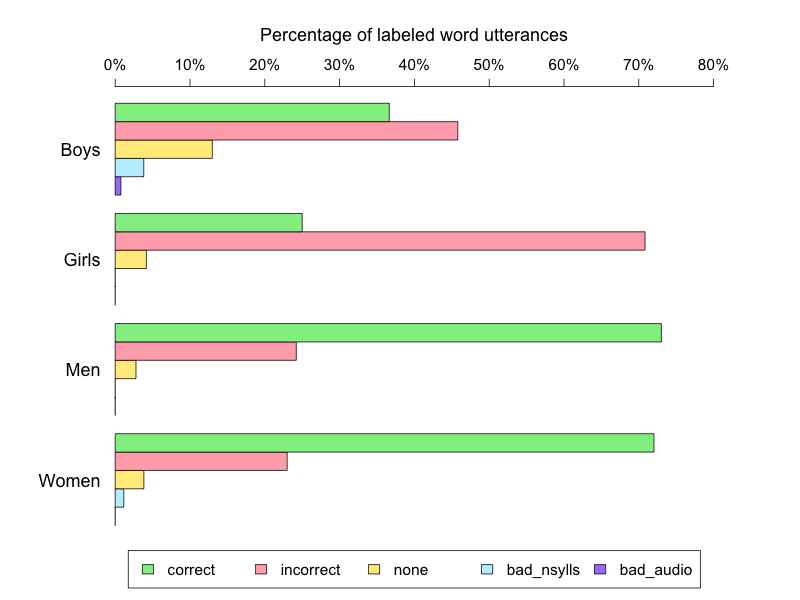
\includegraphics[width=\textwidth]{img/plots/judgmentsAgeGender}
				\end{subfigure}
				
			\end{figure}
			
			\begin{figure}[p]
			\ContinuedFloat
			\centering
				\caption[Error distribution by speaker age and gender (cont.)]{(continued) Distribution of errors by speaker's age and gender,
				as a percentage of the total number of labeled tokens (utterances) from speakers of that age/gender group
				(see \cref{tab:results:agegender} for precise values)
				}
				
				\vspace{1em}
				
				\begin{subfigure}{\textwidth}
					\setcounter{subfigure}{1}
					\centering
					\caption{By age, regardless of gender}
					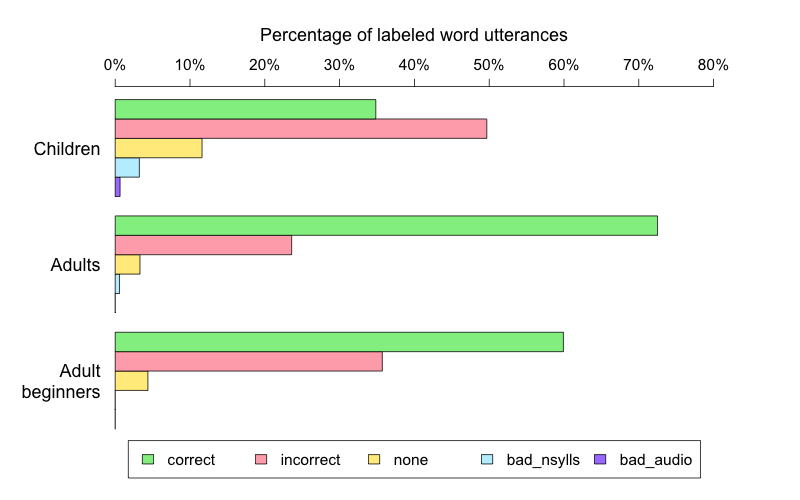
\includegraphics[width=\textwidth]{img/plots/judgmentsAge}
				\end{subfigure}
				
				\vspace{1em}
			
				\begin{subfigure}{\textwidth}
					\centering
					\caption{By gender, regardless of age}
					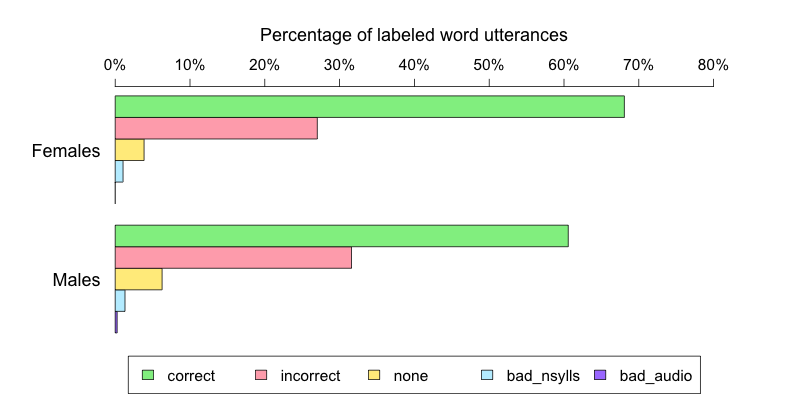
\includegraphics[width=\textwidth]{img/plots/judgmentsGender}
				\end{subfigure}
				
				
				
				\label{fig:results:agegenderbars}
			\end{figure}
		
			
%			\begin{table}[h]
%				\caption[Errors by speaker age and gender]{Errors by speaker age and gender \TODO{add \%ages}}
%				\begin{tabularx}{\textwidth}{XXXXXXXX}			
%				\toprule
%Group	&	correct	&	incorrect	&	none	&	bad\_ nsylls	&	bad\_ audio	&	Total	&	\% of corpus	\\
%				\midrule
%Boys	&	48	&	60	&	17	&	5	&	1	&	131	&	19.61\%	\\
%Girls	&	6	&	17	&	1	&	0	&	0	&	24	&	3.59\%	\\
%Men	&	184	&	61	&	7	&	0	&	0	&	252	&	37.72\%	\\
%Women	&	188	&	60	&	10	&	3	&	0	&	261	&	39.07\%	\\
%
%\midrule		
%Children	&	54	&	77	&	18	&	5	&	1	&	155	&	23.20\%	\\													
%Adults	&	372	&	121	&	17	&	3	&	0	&	513	&	76.80\%	\\
%Adults (A2~only) & 86 & 49 & 9 & 0 & 0 & 144 & 21.56\%\\
%Adults (A2,~B1) &  151 & 90 & 11 & 0 & 0 & 252 & 37.72\%\\
%
%\midrule															
%Females	&	194	&	77	&	11	&	3	&	0	&	285	&	42.66\%	\\
%Males	&	232	&	121	&	24	&	5	&	1	&	383	&	57.34\%	\\
%				\bottomrule	
%				\end{tabularx}
%				\label{tab:results:agegender}
%			\end{table}
			
			
%			\begin{figure}[htb]
%				\centering
%				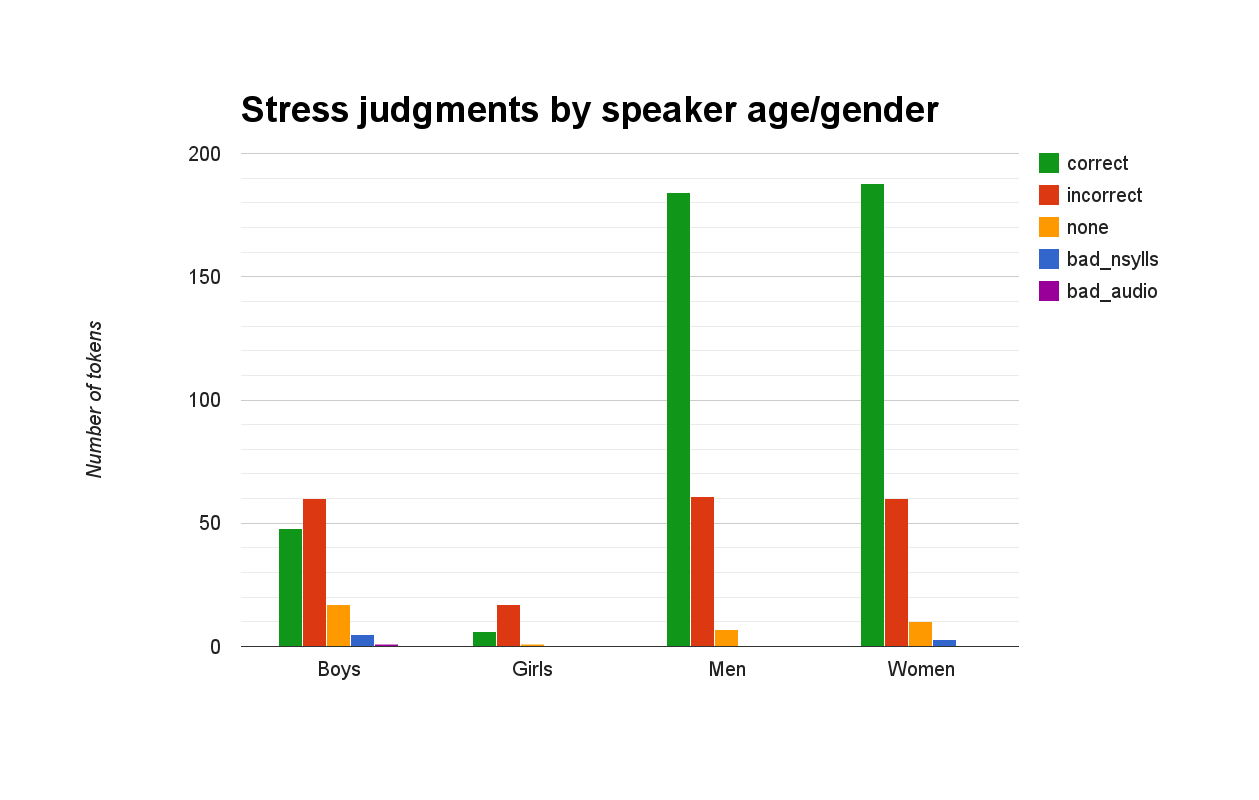
\includegraphics[width=\textwidth]{img/annotation/ageGenderBars}
%				\caption{Stress judgments by speaker age/gender}
%				\label{fig:results:agegenderbars}
%			\end{figure}
%			
			
%			\begin{figure}[htb]
%				\centering
%				\begin{subfigure}[t]{0.5\textwidth}
%					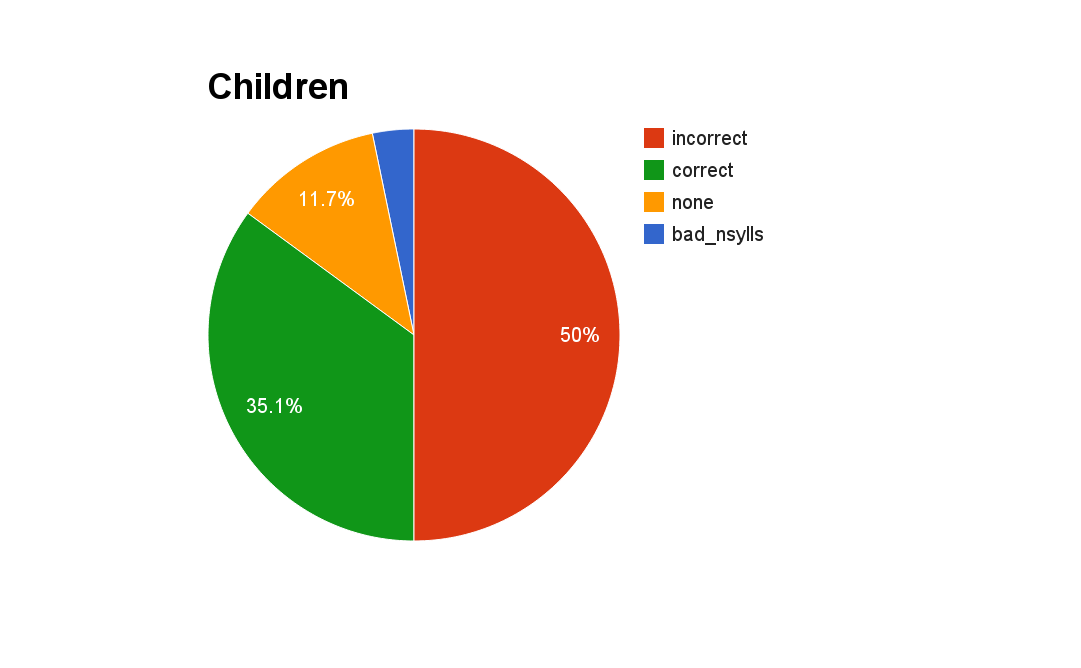
\includegraphics[width=\textwidth]{img/annotation/childPie}
%					\caption{Children}
%					\label{fig:results:agepies:child}
%				\end{subfigure}%
%				~
%%				\begin{subfigure}[t]{0.5\textwidth}
%%					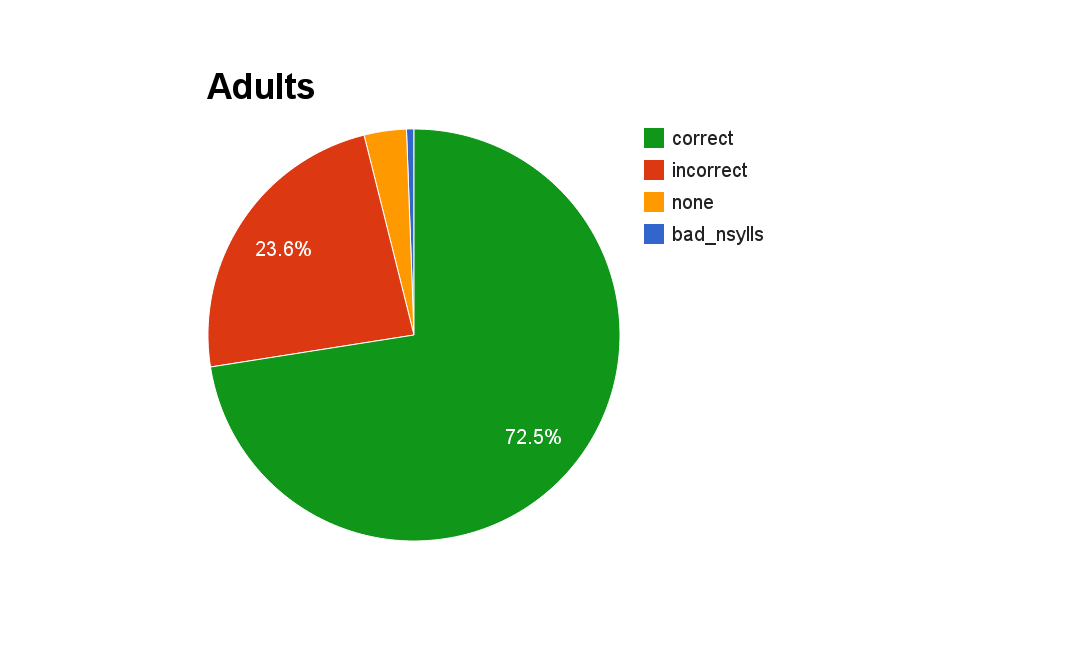
\includegraphics[width=\textwidth]{img/annotation/adultPie}
%%					\caption{Adults \TODO{remove?}}
%%					\label{fig:results:agepies:adult}
%%				\end{subfigure}%
%%		
%				\begin{subfigure}[t]{0.5\textwidth}
%					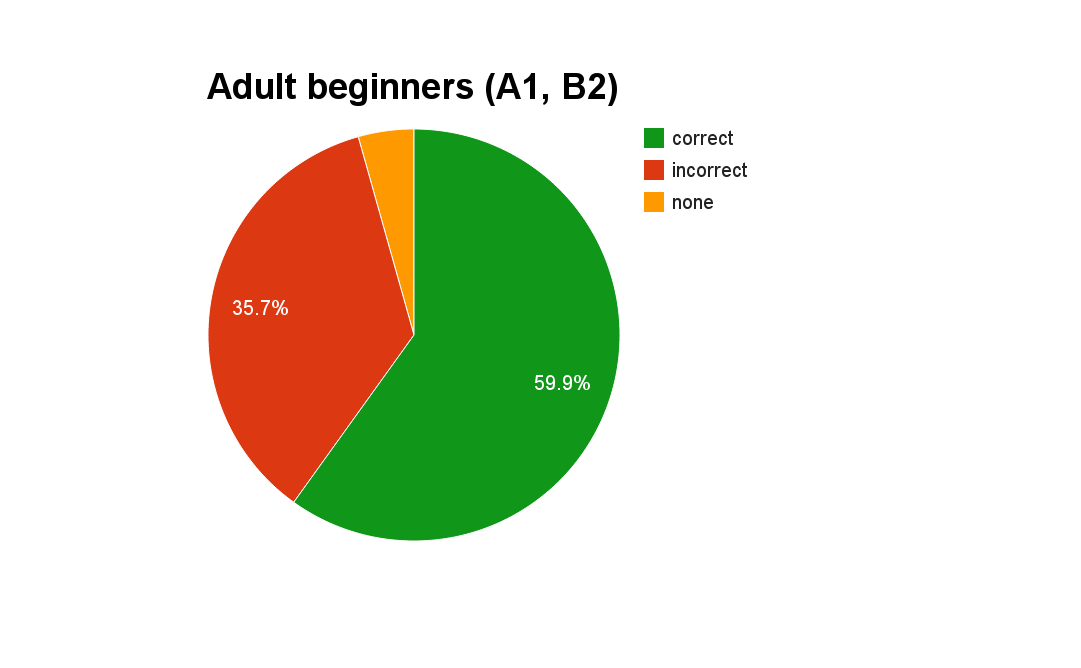
\includegraphics[width=\textwidth]{img/annotation/adultBeginnersPie}
%					\caption{Adult beginners}
%					\label{fig:results:agepies:adultbeg}
%				\end{subfigure}%
%				
%				\caption{Error distribution by speaker age}
%				\label{fig:results:agepies}
%			\end{figure}	
%			
%			\begin{figure}[htb]
%				\centering
%				\begin{subfigure}[t]{0.5\textwidth}
%					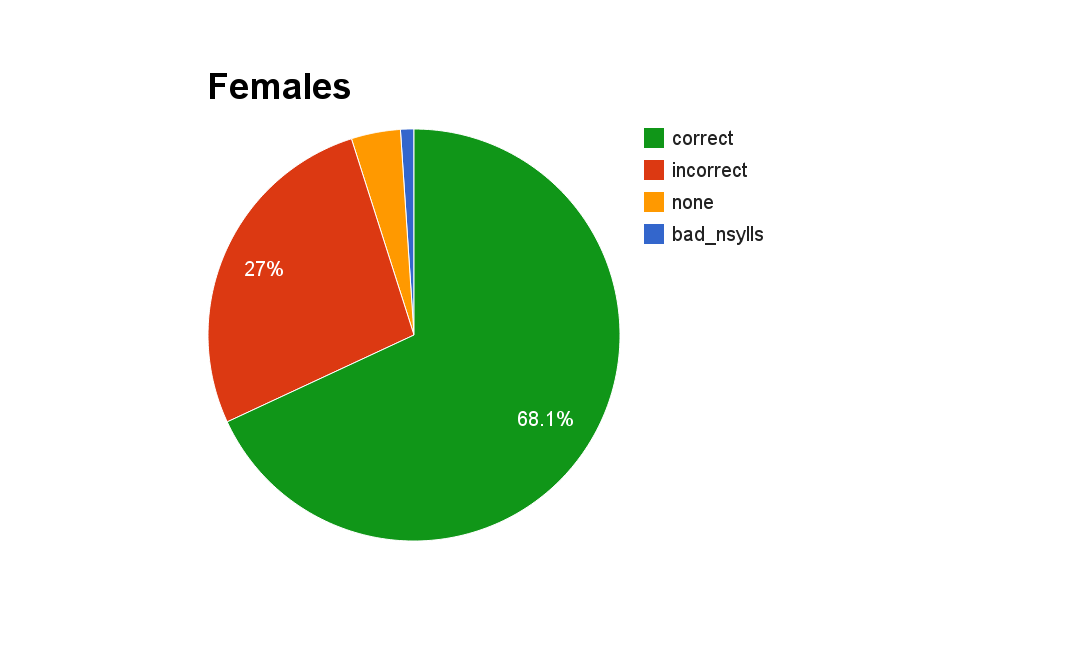
\includegraphics[width=\textwidth]{img/annotation/femalePie}
%					\caption{Females}
%					\label{fig:results:genderpies:female}
%				\end{subfigure}%
%				~
%				\begin{subfigure}[t]{0.5\textwidth}
%					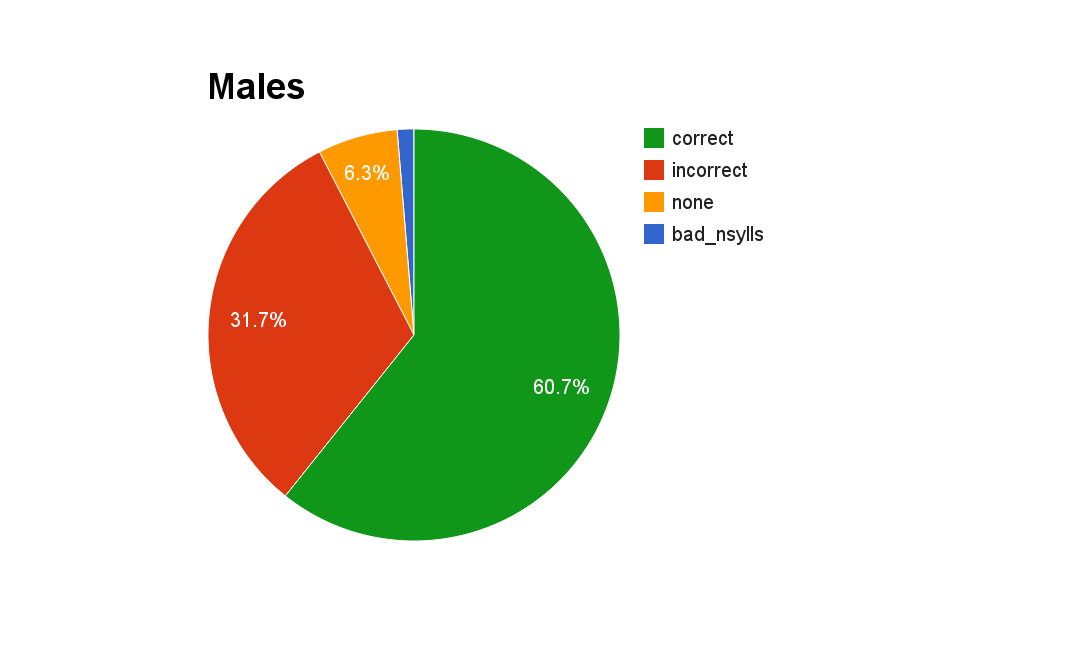
\includegraphics[width=\textwidth]{img/annotation/malePie}
%					\caption{Males}
%					\label{fig:results:genderpies:male}
%				\end{subfigure}%
%				\caption{Error distribution by speaker gender}
%				\label{fig:results:genderpies}
%			\end{figure}	
			
			
			
				
%				\begin{figure}[htb]
%				\centering
%				\begin{subfigure}[t]{0.5\textwidth}
%					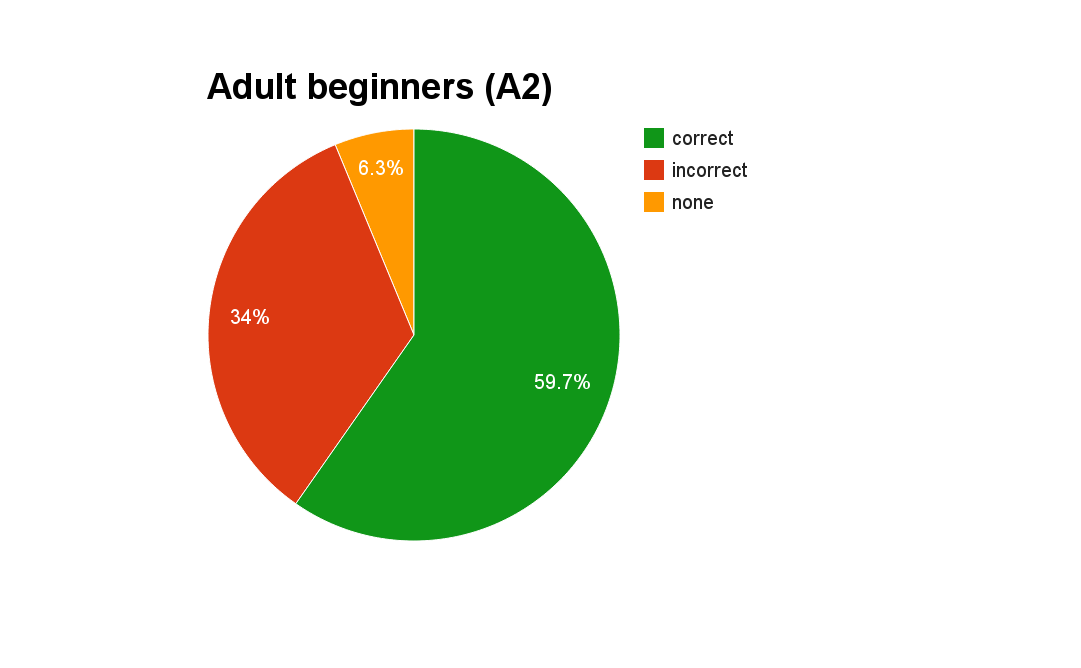
\includegraphics[width=\textwidth]{img/annotation/adultA2Pie}
%					\caption{Adults of A2 skill level}
%					\label{fig:results:adultbeginners:a2}
%				\end{subfigure}%
%				~
%				\begin{subfigure}[t]{0.5\textwidth}
%					\includegraphics[width=\textwidth]{img/annotation/adultBeginnersPie}
%					\caption{Adult beginners (A2 and B1)}
%					\label{fig:results:adultbeginners:a2b1}
%				\end{subfigure}%
%				\caption{Error distribution for adult beginners}
%				\label{fig:results:adultbeginners}
%			\end{figure}	
				
				
		
%		\subsection{Errors by recording condition}
%		\label{sec:results:condition}
%			\TODO{}
%		
%		\begin{table}
%			\centering
%			\caption{Stress judgments by recording condition}
%			\begin{tabular}{lrrrr}
%			\toprule
%	Judgment	&	SH tokens	&	\% of SH	&	SR tokens	&	\% of SR	\\
%	\midrule
%	correct	&	97	&	58.79\%	&	329	&	65.41\%	\\
%	incorrect	&	51	&	30.91\%	&	147	&	29.22\%	\\
%	none	&	14	&	8.48\%	&	21	&	4.17\%	\\
%	bad\_nsylls	&	3	&	1.82\%	&	5	&	0.99\%	\\
%	bad\_audio	&	0	&	0.00\%	&	1	&	0.20\%	\\
%	\midrule
%	Total	&	165	&		&	503	&		\\
%	\% of corpus	&	24.70\%	&		&	75.30\%	&		\\	
%	\bottomrule
%			\end{tabular}
%			\label{tab:results:condition}
%		\end{table}
%		
%		\begin{figure}[htb]
%				\centering
%				\begin{subfigure}[t]{0.5\textwidth}
%					\includegraphics[width=\textwidth]{img/annotation/SRpie}
%					\caption{Sentence Read}
%					\label{fig:results:conditionpies:SR}
%				\end{subfigure}%
%				~
%				\begin{subfigure}[t]{0.5\textwidth}
%					\includegraphics[width=\textwidth]{img/annotation/SHpie}
%					\caption{Sentence Heard}
%					\label{fig:results:conditionpies:SH}
%				\end{subfigure}%
%				\caption{Error distribution by recording condition}
%				\label{fig:results:conditionpies}
%			\end{figure}			
%		
%	
%		\subsection{Impact of technical problems \TODO{remove?}}
%		\label{sec:results:techproblems}
%			\TODO{remove?}
	
	
	\section{Summary}
	\label{sec:lexstress:summary}
	\TODO{}